\chapter{Àlgebra lineal}\label{algebra}
Quan vaig començar a buscar informació sobre computació quàntica, en vaig ràpidament donar compte que necessitava molt més coneixement matemàtic, degut a que no entenia gairebé res dels llibres sobre computació quàntica. Arran aquell temps, una serie de vídeos sobre àlgebra lineal en va captar l’atenció, que es justament la branca de les matemàtiques sobre la qual es basa la computació quàntica. Els vídeos son les lliçons que dona el Professor Gilbert Strang al Institut Tecnològic de Massachusetts (MIT en anglès) \cite{LA_OCW_strang, LA2_OCW_strang}. Una vegada havia vist gairebé tots els vídeos, ja tenia bastants conceptes apresos. 

Aquelles lliçons es van ajudar a entendre les matemàtiques de \textit{Quantum Computation and Quantum Information} \cite{QCandQI} i \textit{Quantum Computing: A Gentle Introduction}. A poc a poc, vaig anar aprenent els fundaments matemàtics de la computació quàntica i mecànica quàntica.

En aquesta secció aniré explicant els conceptes bàsics de l'àlgebra lienal, per formar els coneixements en matemàtiques necessaris per poder comprendre aquest treball. 

\section{Vectors i espais vectorials}
Els objectes fonamentals de l'àlgebra lineal són els espais vectorials. Un espai vectorial es el conjunt de tots els vectors que tenen les mateixes dimensions. Per exemple  $\mathbb{R}^{3}$ seria el espai vectorial de tots els vectors de 3 dimensions, aquests vectors normalment s'utilitzen per representar punts en un espai tridimensional. En computació quàntica un tipus d'espais vectorials en concret són utilitzats: Els espais de Hilbert, en altres paraules, un espai vectorial amb un producte interior \cite{QCandQI:GramSchmidt}. Els espais de Hilbert segueixen un conjunt de productes i compleixen unes certes normes, en aquest capítol presentaré una part d'aquestes normes i productes, la quantitat que és necessària. S'ha de tenir en compte que els espais de Hilbert són molt més complicats que el que es representa en aquest treball, també que d'aquí en endavant, quan mencioni espai vectorial hem referiré a un espai de Hilbert, d'ha no ser que s'especifiqui el contrari. 

Els espais vectorial estan definits per les seves bases, un set de vectors $B = \{\ket{v_1}, \dots, \ket{v_n}\}$ es una base vàlida per l'espai $V$, si cada vector $\ket{v}$ en l'espai es pot escriure com $\ket{v} = \sum_i a_i \ket{v_i}$ per $\ket{v_i} \in B$. Els vectors de la base $B$ són linealment independent entre ells.

La notació estàndard pels conceptes de  àlgebra lienal en mecànica quàntica es la notació de Dirac, en la qual es representa un vector com $ \ket{\psi} $. On $\psi$ es la etiqueta del vector. Un vector $ \ket{\psi} $ amb $n$ dimensions també pot ser representat com una matriu columna que te la forma: 
$$
\ket{\psi} = 
\begin{bmatrix}
	z_{1} \\
	z_{2} \\
	\vdots \\
	z_{n-1} \\
	z_{n}
\end{bmatrix}
$$

On els nombres complexes $(z_{1}, z_{2}, \dots , z_{n-1}, z_{n} )$ són els seus elements. Un vector escrit com a $\ket{\psi}$ també s'anomena \textit{ket}.

La adició d'un par de vectors en un espai de Hilbert es definida per \footnote{Els vectors d'aquesta definició tenen els seus elements representats per la seva etiqueta i un subscrit e.g. el vector $\ket{\psi}$ te un element qualsevol $\psi_{1}$ i el seu primer element es $\psi_{1}$. Aquesta notació es seguirà utilitzant al llarg del treball.}:
$$
\ket{\psi} + \ket{\varphi} = \begin{bmatrix} \psi_{1} \\ \vdots \\ \psi_{n} \end{bmatrix} +
\begin{bmatrix} \varphi_{1} \\ \vdots \\ \varphi_{n} \end{bmatrix}
$$

A més a més, hi ha una multiplicació per un escalar\footnote{Un numero qualsevol en $\mathbb{R}$.} definida per:
$$
  z\ket{\psi} = z\begin{bmatrix} \psi_{1} \\ \vdots \\ \psi_{n} \end{bmatrix} = \begin{bmatrix} z \psi_{1} \\ \vdots \\ z \psi_{n} \end{bmatrix}
$$
On $z$ es un escalar i $\ket{\psi}$ un vector. Cal que notar que cada element del vector es multiplicar per el escalar.

Degut a que els espais de Hilbert son complexos tenen un conjugat complex definit per escalar com a: Per un escalar complex $z=a +bi$, el seu conjugat $z^*$ es igual a $a-bi$. 

Aquesta noció pot ampliar per a vectors i matrius, agafant el conjugat de totes els seus elements:
$$
\ket{\psi}^{*} = 
	\begin{bmatrix} \psi_{1} \\ \vdots \\ \psi_{n} \end{bmatrix}* = \begin{bmatrix} \psi_{1}^* \\ \vdots \\ \psi_{n}^* \end{bmatrix}
$$
$$
A^{*} = 
	\begin{bmatrix} 
	a_{11} & \cdots & a_{1n}\\ 
	\vdots & \ddots & \vdots \\ 
	a_{m1} & \cdots & a_mn
\end{bmatrix}^* 
= \begin{bmatrix} 
	a_{11}^* & \dots & a_{1n}^*\\ 
	\vdots & \ddots & \vdots \\ 
	a_{m1}^* & \cdots & a_mn^*
\end{bmatrix}
$$
Amb $\ket{\psi}$ sent un vector de dimensions $n$, i $A$ sent una matriu de dimensions $m \times n$.

Un altre concepte important es la transposada, representada per el superíndex $T$ que 'rota' un vector o una matriu. Un vector columna amb una dimensió $n\times 1$ es transforma amb un vector fila amb una dimensió $1\times n$\footnote{En realitat els vectors columna son matrius amb dimensió $n,1$ però he estat ometent el 1. Quan hem refereixo a les dimensions de un vector qualsevol, només diré un numero, no obstant, especificaré si és un vector columna o un vector fila.}:
$$
\ket{\psi}^{T} = 
	\begin{bmatrix} \psi_{1} \\ \vdots \\ \psi_{n} \end{bmatrix}^T = \begin{bmatrix} \psi_{1} & \dots & \psi_{n} \end{bmatrix}
$$

El mateix és cert per les matrius, una matriu $m\times n$ transposada es converteix en una matriu $n \times m$. Per exemple:
$$
A^T = \begin{bmatrix}
	 2 & 3 \\
	 6 & 4 \\
	 2 & 5 
\end{bmatrix}^T = \begin{bmatrix}
 2 & 6 & 2 \\
 3 & 4 & 5
\end{bmatrix}
$$

La composició d'un conjugat complex i la transposada s'anomena el conjugat Hermitià, la seva notació es una $\dagger$ superindexada. Per un vector $\ket{\psi}$ el seu conjugat Hermitià $\ket{\psi}^\dagger$ és:
$$
\ket{\psi}^\dagger = (\ket{\psi}^*)^T =  \begin{bmatrix} \psi_{1}^* & \dots & \psi_{n}^* \end{bmatrix} = \bra{\psi}
$$
El conjugat Hermitià compleix que $\ket{\psi}^\dagger = \bra{\psi}$ i $\bra{\psi}^\dagger = \ket{\psi}$.

El conjugat Hermitià d'un vector columna $\ket{\psi}$ s'anomena \textit{bra} o vector dual. En la notació de Dirac un vector dual s'escriu com $\bra{\psi}$.

\section{Aplicacions lineals}
Per poder operar amb vectors i fer operacions amb ells, s'utilitzen les matrius, que també son anomenades aplicacions lineal o transformacions lineals\footnote{}, que són noms que descriuen millor com funcionen aquests objectes. La definició formal d'una aplicació lienal pot ser bastant complicada, per aquesta raó, utilitzaré termes més informals en aquesta secció. 

Bàsicament, una aplicació lineal transforma un vector en un altre vector, que poden o no ser d'espais diferents \cite{LR_done_right:linear_map}. Més formalment, per un vector $\ket{v}$ en un espai $V$ i un vector $\ket{w}$ en un espai $W$, una transformació lineal $A$ entre els vectors, fa l'acció:
$$
A \ket{v} = \ket{w}
$$
En altres paraules, l'aplicació transforma un element del espai vectorial $V$ en un vector del espai vectorial $W$.
Les transformacions lienals han de complir les següents propietats:
\begin{enumerate}
	\item Addició de vectors: \\
	Donats els vectors $\ket{\psi}$ i $\ket{\varphi}$ en un mateix espai vectorial, i un operador lineal $A$:
	$$ A(\ket{\psi} + \ket{\varphi}) = A\ket{\psi} + A\ket{\varphi}$$ 
	\item Producte escalar:\\
	Donats els vectors $\ket{\psi}$, l'escalar $z$ i la transformació lienal $A$, es certs que:
	$$ A(z\ket{\psi}) = z A \ket{\psi}$$
\end{enumerate}

Aquestes afirmacions han de ser certes per tots els vectors i tots els escalars en els espais on les aplicacions actuen. Cal notar que una aplicació lineal no té perquè ser una matriu necessàriament, per exemple, les derivades i les integrals son aplicacions lineals, això es pot provar fàcilment al veure que compleixen els criteris especificats posteriorment. No obstant, les derivades i les integrals usualment no s'apliquen a vectors, sinó a les funcions, però es possible aplicar-les a vectors \footnote{No et preocupis, que es clar que les aplicaré a vectors :D.}.

Les matrius només són la representació matricial de les aplicacions lineals \cite{LR_done_right:matrix}.

	\subsection{Tipus d'aplicacions lineals}
En la secció actual, exposaré els tipus bàsics d'aplicacions lineals que són indispensables en la teoria presentada en aquest capítol i la rest del treball.

\begin{enumerate}
	\item \textbf{Operador zero} \\
	Qualsevol espai vectorial té un vector zero expressat en notació de Dirac com a $0$, degut a que $\ket{0}$ es un altre concepte totalment diferent en CQ i IQ\footnote{Computació Quàntica i Informació Quàntica.}. El vector zero es aquell vector que per qualsevol vector $\ket{\psi}$ i qualsevol escalar $z$, es compleix que:	
	$\ket{\psi} + 0 = \ket{\psi} $ i $z0 = 0$. \\
	El operador zero també s'escriu com a $0$ i es defineix com l'aplicació que transforma qualsevol vector al vector zero: $0\ket{\psi} = 0 $.  
	
	\item \textbf{Matriu inversa} \\
	Un matriu quadrada\footnote{Una matriu quadrada és una matriu amb dimensions $n\times n$, on $n \in \mathbb{N}$.} $A$ és invertible si existeix una matriu $A^{-1}$ de manera que $AA^{-1}=A^{-1}A$. $A^{-1} = I$ és la matriu inversa de $A$. La manera més ràpida de saber si una matriu es invertible es veient si el seu determinant no és zero. En altres paraules, és l'element neutre per la suma i l'element null per la multiplicació. 

	\item \textbf{Matriu Identitat} \\
	Per a qualsevol espai vectorial $V$ existeix un operador identitat $I$ que es definit com $I\ket{\psi} = \ket{\psi}$, aquest operador no fa cap canvi al vectors als quals opera. Cal notar també que per qualsevol matriu $A$ i la seva inversa és veritat que $AA^{-1} = I$. 
	
	\item \textbf{Matriu Unitari} \\
	Un operador unitari es qualsevol operador que no altera la norma dels vectors al quals es aplicat, per tant, una matriu es unitària si $AA^\dagger = I$
	Per convertir qualsevol operador en unitari, es divideix les seves entrades entre la norma del operador. 
	
	\item \textbf{Matrius Hermitianes} \\
	Una matriu Hermitiana compleix que: 
	$$
	\bra{\psi} (A \ket{\varphi}) = (A^\dagger\bra{\psi})\ket{\varphi}
	$$
	On $\ket{\psi}$ i $\ket{\varphi}$, són dos vectors del espai en el qual actua $A$. Si apliquem el producte interior a aquesta equació tenim que: $A = A^\dagger$.
	
\end{enumerate}

\section{Producte interior i producte exterior}

\subsection{Producte interior}
Un vector dual $\bra{\psi}$ i un vector $\ket{\varphi}$ combinats formen el producte interior $\bra{\psi}\ket{\varphi}$, el qual efectua una operació que agafa els dos vectors com a input i produeix un nombre complex com a output:
$$
\bra{a}\ket{b} = a_1 b_1 + a_2 b_2 + ... + a_{n-1} b_{n-1} + a_n b_n = z
$$
Amb $z, a_i, b_i \in \mathbb{C}$. Quan hem refereixo a un producte interior, normalment diré "el producte interior de dos vectors", quan en realitat es una operació entre un vector dual i un vector.

El equivalent d'aquest producte en un espai real de dos dimensions $\mathbb{R}^2$ és el producte escalar, que s'expressat com a :
\begin{equation}
	\bra{a}\ket{b} = \norm{\ket{a}}_2 \cdot \norm{\ket{b}}_2 \cos \theta 
	\label{eq:dot_product}
\end{equation}


Amb $\norm{\cdot}_2$ sent la norma $\ell^2$  definida com a $\norm{\ket{\psi}}_2 = \sqrt{\psi_{1}^2 + \cdots + \psi_{n}^2}$ amb $\theta$ sent l'angle entre els vectors $\ket{a}$ i $\ket{b}$. Com he dit l'equació \eqref{eq:dot_product} és equivalent al producte interior, no obstant, segons el que he vist, no es usada àmpliament ja que interpretar $\theta$ com un angle entre vectors de dimensions altes no té molt de sentit. En contrast, he vist aquest producte presentat en la seva interpretació geomètrica\footnote{Els detalls exactes de l'interpretació geomètrica estan fora del domini d'aquest treball, malgrat que m'agradaria molt parlar sobre el tema.} com el producte entre un vector fila i un vector columna: 
% The Geometry of Linear Equations: https://www.youtube.com/watch?v=ZK3O402wf1c&list=PL3CCC70370BD3FD48&index=1
% The four Fundamental Subspaces: https://www.youtube.com/watch?v=nHlE7EgJFds
$$
\bra{a}\ket{b} = \begin{bmatrix}a_1  \cdots  a_n \end{bmatrix} \begin{bmatrix} b_{1} \\ \vdots \\ b_{n} \end{bmatrix}
$$

Ja he definit la norma $\ell_2$ com l'arrel quadrada de la suma del elements d'un vector al quadrat:
$$
\norm{\ket{a}}_2 = \sqrt{\sum_{i} \abs{a_{i}}^2}
$$
No obstant, la definició més comú es basa en el producte interior. Com es pot veure el producte interior de un vector per ell mateix es la suma de les seves entrades al quadrat:
$$
\bra{a}\ket{a} = a_1 a_1 + \cdots + a_n a_n = a_1^2 + \cdots +  a_n^2 \\= \sum_{i} \abs{a_i}^2
$$
Per tant, la norma pot ser definida com l'arrel quadrada del producte interior d'un vector:
\begin{equation}
\norm{\ket{a}}_2 = \sqrt{\bra{a}\ket{a}}
\label{eq:norm}
\end{equation}
Quan la norma es aplicada a un vector bidimensional, es pot veure que es lo mateix que la longitud Euclidiana d'aquell vector, això es perquè realment son el mateixos conceptes, tot i això, la norma es el concepte de longitud però generalitzat a vectors de dimensions altes. 

Pel el que jo entenc algunes propietats de la longitud d'un vector bidimensional no es mantenen amb la norma d'un vector que te més de 2 dimensions. En altres paraules, la norma es comporta en certes maneres com la distancia des de d'origen (que es la definició de la longitud), per tant, no són exactament lo mateix. A més d’això, hi han diferents tipus de normes que s'utilitzen en diversos escenaris. Aquesta es la raó per la qual en refereixo a la norma, com la norma $\ell^2$. A aquesta norma també se li diu norma Euclidiana \cite{wolfram:2norm}.

\subsubsection{Propietats del producte interior}
Les propietats bàsiques del producte interior són les següents:
\begin{enumerate}
	\item És lineal en el segon argument $ (z_1\bra{a}+ z_2\bra{c})\ket{b} = z_1\bra{a}\ket{b} + z_2\bra{c}\ket{b}$
	\item Té simetria en el conjugat $\bra{a}\ket{b} = (\bra{b}\ket{a})^*$
	\item $\bra{a}\ket{a}$ es no-negativa i real, excepte en el cas de $\bra{a}\ket{a} = 0 \Leftrightarrow \ket{a} = 0$
\end{enumerate}

 
\subsection{Vectors ortonormals i ortogonals}
A partir del concepte de norma sorgeixen els conceptes de un par de vectors ortonormals i un par de vectors ortogonals \footnote{Una nota graciosa, la primera vegada que vaig trobar aquest dos conceptes els vaig confondre i pensava que eren la mateixa cosa, això hem va confondre moltíssim i no entenia gairebé res.}.
Mirant l'equació \eqref{eq:norm} podem veure que si el producte interior del vector és 1, la norma del mateix vector també és 1. Un vector que té norma 1, és un vector unitari. D'aquesta manera, si el producte interior d'un vector és 1, és un vector unitari. 

De vectors que no són zero son ortogonals si el seu producte interior és zero. Si aquests vectors són de bidimensionals, a partir de l'equació \eqref{eq:dot_product} podem veure que l'angle que fan entre ells és zero i per tant son perpendiculars entre ells: 
\begin{multline*}
	 \text{Per }\ket{a} \text{i} \ket{b}\neq 0 : \\
	\text{Si }\bra{a}\ket{b} = 0 \text{ tenim que: } \norm{\ket{a}}_2 \cdot \norm{\ket{b}}_2 \cos \theta = 0 \\
	 \text{Perquè $\ket{a}$ i $\ket{b}$ no son zero, les seves normes no són zero.} \\
	 \text{Per tant el terme que falta } \cos\theta \text{ és igual a zero.} \\
	 \text{D'aquesta manera, l'angle $\theta$ ha de ser } \frac{\pi}{2}. \\
\end{multline*}
No obstant, pensar que la perpendicularitat i la ortogonalitat són els mateixos conceptes es un error, degut a que, el que siguin només es veritat per els vectors bidimensionals. Perquè com en el cas de la norma i la longitud, la ortogonalitat és el concepte de perpendicularitat generalitzat. 

Quan barregem els conceptes de vector unitari i vectors ortogonals arribem a la ortonormalitat \cite{QCandQI:GramSchmidt}. Un parell de vectors que no són zero, són ortogonals quan els dos són unitaris i també són ortogonals entre ells:

$$
\ket{a} \text{and } \ket{b} \text{ son ortonormals si:} \left\{
	\begin{array}{ll}
		\bra{a}\ket{b} = 0 \\
		\bra{a}\ket{a} = 1 \\
		\bra{b}\ket{b} = 1 \\
	\end{array}
\right.
$$
Els vectors ortonormals són importants, àmpliament utilitzats tant en computació quàntica com en mecànica quàntica perquè serveixen per crear bases vectorials molt útils. 

Una altre cosa que remarcar i no he dit es que al dir un par de vectors, aquest par també pot ser un set de vectors. Si un set té tots els vectors unitaris i ortogonals entre tots ells, és un set de vectors ortonormals. 
El set de vectors $ B = \{\ket{\beta_1}, \ket{\beta_2}, ..., \ket{\beta_{n-1}} \ket{\beta_n}\} $ és ortonormal si $\bra{\beta_i}\ket{\beta_j} = \delta_{ij}  \forall i, j$ \cite{QCandQI:GramSchmidt} on $\delta_{ij}$ és el Kronecker delta, definit com:
: 
$$
\delta_{ij} =
\begin{cases}
	1 &\text{si } i=j\\
	0 &\text{si } i\neq j
\end{cases}
$$

\subsection{Producte exterior}
El producte exterior és una funció (expressada com $\ket{a}\bra{b}$, amb $\ket{a}$ i $\ket{b}$ sent vectors) que agafa dos vectors i produeix un operador lineal com output. Al contrari que el producte interior, no hi ha un producte equiparable en les matemàtiques ensenyades al institut, i és una mira difícil d'entendre perquè agafa dos vectors que poden ser d'un espai diferent com input.
És definit com: 

%For a vector $\ket{v}$ and $\ket{v'}$ in the Hilbert space $V$ and a vector $\ket{w}$ in the Hilbert space $W$. The output is a linear operator of dimensions $m \times n$ in the space $M_{m\times n}$:
%$$\ket{v}\bra{w} : V,W \mapsto M_{m\times n} \\ $$
Pels vectors $\ket{v}$ i $\ket{v'}$ amb dimensions $m$ i el vector $\ket{w}$ de dimensió $n$. El producte exterior és l'aplicació lineal $A$ de dimensions $m \times n$ en l'espai $\mathrm{Mat}_{m\times n}$:
$$
\ket{v}\bra{w} = A \text{ with } A\in \mathrm{Mat}_{m\times n} .
$$ 
%In other words, that takes a vector from $\mathbb{C}_i$ to $\mathbb{C}_j$. 
Amb la seva acció definida per: 
\begin{equation}
	(\ket{v}\bra{w})\ket{v'} \equiv \ket{w}\bra{v}\ket{v'} = \bra{v}\ket{v'}\ket{w}
	\label{eq:outer_def}
\end{equation}

A partir de l'equació \eqref{eq:outer_def} l'utilitat i significat del producte es bastant complicada d'entendre, per tant exposaré la manera de computar-lo per clarificar com funciona. Per dos vectors $\ket{a}$ i $\ket{b}$ de dimensions $m$ i $n$ respectivament, el seu producte interior es computa multiplicant cada element de $\ket{a}$ per cada elment de $\ket{b}$ formant una matriu amb mida $m\times n$:
$$
\ket{a}\bra{b} = \begin{bmatrix}
	a_1 b_1 & a_1 b_2 & \cdots & a_1 b_n \\
	a_2 b_1 & a_2 b_2 & \cdots & a_2 b_n \\
	\vdots  & \vdots  & \ddots& \vdots  \\
	a_m b_1 & a_m b_2 & \cdots & a_m b_n \\
\end{bmatrix}
$$
L'utilitat d'aquest producte és mostrara més endavant.

\section{Producte tensorial}
L'últim producte que mencionaré és el tensorial, representat per el símbol $\otimes$. Aquest producte s'utilitza per crear espais vectorials més grans combinant espais vectorials més petits. La definició formal és bastant complicada, per tant en centraré en explicar la manera amb la qual es computa utilitzant la representació matricial d'aquest producte, anomenada el producte de Kronecker. 

Per una $m \times n$ $A$, i una $p \times q$ matriu $B$, el seu producte de Kronecker \cite{QCandQI:kronecker} és la matriu de mida $pm \times qn$: 
\begin{multline*}
A \otimes B = \begin{bmatrix}
	a_{11} B & a_{12} B & \cdots & a_{1n}B \\
	a_{21} B & a_{22} B & \cdots & a_{2n}B \\
	\vdots & \vdots & \ddots &           \vdots \\
	a_{m1} B & a_{m2} B & \cdots & a_{mn} B
\end{bmatrix} \\
= \begin{bmatrix}
a_{11} b_{11} & a_{11} b_{12} & \cdots & a_{11} b_{1q} &
\cdots & \cdots & a_{1n} b_{11} & a_{1n} b_{12} & \cdots & a_{1n} b_{1q} \\
a_{11} b_{21} & a_{11} b_{22} & \cdots & a_{11} b_{2q} &
\cdots & \cdots & a_{1n} b_{21} & a_{1n} b_{22} & \cdots & a_{1n} b_{2q} \\
\vdots & \vdots & \ddots & \vdots & & & \vdots & \vdots & \ddots & \vdots \\
a_{11} b_{p1} & a_{11} b_{p2} & \cdots & a_{11} b_{pq} &
\cdots & \cdots & a_{1n} b_{p1} & a_{1n} b_{p2} & \cdots & a_{1n} b_{pq} \\
\vdots & \vdots & & \vdots & \ddots & & \vdots & \vdots & & \vdots \\
\vdots & \vdots & & \vdots & & \ddots & \vdots & \vdots & & \vdots \\
a_{m1} b_{11} & a_{m1} b_{12} & \cdots & a_{m1} b_{1q} &
\cdots & \cdots & a_{mn} b_{11} & a_{mn} b_{12} & \cdots & a_{mn} b_{1q} \\
a_{m1} b_{21} & a_{m1} b_{22} & \cdots & a_{m1} b_{2q} &
\cdots & \cdots & a_{mn} b_{21} & a_{mn} b_{22} & \cdots & a_{mn} b_{2q} \\
\vdots & \vdots & \ddots & \vdots & & & \vdots & \vdots & \ddots & \vdots \\
a_{m1} b_{p1} & a_{m1} b_{p2} & \cdots & a_{m1} b_{pq} &
\cdots & \cdots & a_{mn} b_{p1} & a_{mn} b_{p2} & \cdots & a_{mn} b_{pq}
\end{bmatrix}
\end{multline*}

Cal tenir en compte que $a_{ij}B$ es una multiplicació escalar per una matriu, amb $a_{ij}$ sent l'escalar i $B$ sent la matriu. 

Aquí hi ha un exemple més il·lustratiu amb dues matrius de mida $2\times2$, es pot veure que cada element de la primera matriu es multiplicat per la segona matriu:
\begin{equation*}
\begin{bmatrix}
	1 & 2 \\
	3 & 4 \\
\end{bmatrix} \otimes
\begin{bmatrix}
	0 & 5 \\
	6 & 7 \\
\end{bmatrix} =
\begin{bmatrix}
1 \begin{bmatrix}
	0 & 5 \\
	6 & 7 \\
\end{bmatrix} & 
2 \begin{bmatrix}
	0 & 5 \\
	6 & 7 \\
\end{bmatrix} \vspace{6pt} \\ 
3 \begin{bmatrix}
	0 & 5 \\
	6 & 7 \\
\end{bmatrix} & 
4 \begin{bmatrix}
	0 & 5 \\
	6 & 7 \\
\end{bmatrix}
\end{bmatrix}
\end{equation*}

\begin{equation*}
	= 
\begin{bmatrix}
1\times 0 & 1\times 5 & 2\times 0 & 2\times 5 \\
1\times 6 & 1\times 7 & 2\times 6 & 2\times 7 \\
3\times 0 & 3\times 5 & 4\times 0 & 4\times 5 \\
3\times 6 & 3\times 7 & 4\times 6 & 4\times 7 \\
\end{bmatrix} \\
= 
\begin{bmatrix}
0 &  5 &  0 & 10 \\
6 &  7 & 12 & 14 \\
0 & 15 &  0 & 20 \\
18 & 21 & 24 & 28
\end{bmatrix}
\end{equation*}

Una altre notació a tenir en compte és el símbol $\bigotimes$, utilitzat per representar el equivalent de la suma (expressada amb $\sum$), però en comptes de la adició el producte de Kronecker és utilitzat. En altres paraules, $\bigotimes$ representa el producte de Kronecker de un nombre finit de termes. Per clarificar, aquí hi ha un exemple amb una matriu identitat: 

Amb $\mathbb{I}$ com la matriu $\begin{bmatrix} 1 & 0 \\ 0 & 1 \end{bmatrix}$ i $n$ com una potencia de $2$:
$$
\mathbb{I}_n = \bigotimes^{\log_{2} n} \mathbb{I}  
$$
	
Aquí està el cas per $n=8$: 
$$\mathbb{I}_8 =  \bigotimes^{\log_{2} 8} \mathbb{I} =\bigotimes^3 \mathbb{I} = \mathbb{I} \otimes \mathbb{I} \otimes \mathbb{I} =
	\begin{bmatrix}
		1 &0 &0 &0 &0 &0 &0 &0 \\
		0 &1 &0 &0 &0 &0 &0 &0 \\
		0 &0 &1 &0 &0 &0 &0 &0 \\
		0 &0 &0 &1 &0 &0 &0 &0 \\
		0 &0 &0 &0 &1 &0 &0 &0 \\
		0 &0 &0 &0 &0 &1 &0 &0 \\
		0 &0 &0 &0 &0 &0 &1 &0 \\
		0 &0 &0 &0 &0 &0 &0 &1 \\
	\end{bmatrix} 
$$

El producte de Kronecker també funciona amb vectors de la mateixa manera, però amb una multiplicació de escalar per vector.

Per els vectors $\ket{\psi}$ i $\ket{\varphi}$ de dimensions $n$ i $m$ respectivament:
$$
\ket{\psi} \otimes \ket{\varphi} = \begin{bmatrix}
	\psi_{1} \ket{\varphi} \\
	\psi_2 \ket{\varphi} \\
	\vdots \\
	\psi_{m} \ket{\varphi}
\end{bmatrix} = 
\begin{bmatrix}
\psi_{1} \varphi_1 \\
\psi_{1} \varphi_{2} \\
\vdots \\
\psi_{1} \varphi_{m} \\
\vdots \\
\vdots \\
\psi_{n} \varphi_1 \\
\psi_{n} \varphi_{2} \\
\vdots \\
\psi_{n} \varphi_{m} \\
\end{bmatrix}
$$

S'ha de tenir en compte que el producte de Kronecker també es pot fer entre un vector i una matriu, o viceversa, no obstant, no és molt comú fer-ho.
\todo{page 34 of QC-intro, inner product for a space $V\otimes W$ }
%With $V$ and $W$ being vector spaces of dimension $m$ and $n$ respectively, the tensor product between them $V \otimes W$ is a vector spaces of dimension $mn$. The elements on the space $V \otimes W$ are 
%For the orthonormal basis $\ket{i}$ and $\ket{j}$ of $V$ and $W$ respectively the orthonormal basis for $V\otimes W$ would be $\ket{i}\otimes\ket{j}$.


\subsection{Propietats del producte tensorial}
Les propietats bàsiques del producte tensorial són les següents \cite{QCandQI:tensor_product, wiki:tensor_product}:
\begin{enumerate}
	\item Associativitat: \\ $A \otimes (B + C) = A \otimes B + A \otimes C$ \\
	$ (zA) \otimes B = A \otimes (zB) = z(A \otimes B)$\\
	$ (A \otimes B) \otimes C = A \otimes (B\otimes C)$ \\
	$A \otimes 0 = 0 \otimes A = 0 $
	\item No-commutativitat \footnote{Una cosa guay es que $A \otimes B$ i $B \otimes A$ són 
	permutativament equivalents: \\ $\exists P, Q \Rightarrow A \otimes B = P (  B \otimes A )Q$ on $P$ i $Q$ són matrius permutatives.  }: \\
	$A \otimes B \neq B \otimes A $
\end{enumerate}



%$$
%f: \mathbb{R} \rightarrow \mathbb{R} \text{ or } \mathbb{R} \stackrel{f}{\to} \mathbb{R} 
%$$
%Where $\mathbb{R}$ is the space of all real number, and $\rightarrow$ is 


\section{Traça}
La traça d'una matriu és tal sols la suma dels seus elements en la diagonal principal, la diagonal que va d'abaix a dalt i d'esquerra a dreta.  

Aquí hi ha una matriu $A$ amb la seva diagonal principal marcada:
$$A = 
	\begin{bmatrix}
		\tikzmarktrace{top}{1} & \tikzmarktrace{top2}{1} & 0 \\
		0 & 1 & \tikzmarktrace{bottom2}{1} \\
		\tikzmarktrace{end}{1} & 0 & \tikzmarktrace{bottom}{1}\\
	\end{bmatrix}
$$
\begin{tikzpicture}[overlay,remember picture]
	\draw[opacity=.4,line width=3mm,line cap=round] (top.center) -- (bottom.center);
\end{tikzpicture}

I la seva traça, representada per $\Tr[A]$ és:
$$
\Tr[A] = 1 + 1 + 1 = 3
$$
Més formalment, la traça d'una matriu quadrada $n$-dimensional és:
$$
\Tr[A] = \sum_{i=1}^{n} a_{ii} = a_{11} + a_{22} + \cdots + a_{nn}
$$

La traça d'una matriu té les propietats següents:
\begin{enumerate}
	\item Operador lineal: \\
	Degut a que la traça és un mapa lienal, es compleix que:\\
	$\Tr[A+B] = \Tr[A] + \Tr[B]$ i $\Tr[zA] = z \Tr[A]$, per a totes les matrius quadrades $A$ i $B$, i tots els escalars $z$.
	\item Traça d'un producte tensorial: \\
	$\Tr[A \otimes B] = \Tr[A]\Tr[B]$
	\item La transposada té la mateixa traça: \\
	$\Tr[A]=\Tr[A^T]$
	\item La traça d'un producte és cíclica: \\
	Per una matriu $A$ amb mida $m \times n$ i una matriu $B$ de la mateixa mida:\\
	$\Tr[AB]=\Tr[BA]$
\end{enumerate}

Una altre manera molt útil de computar la traça d'un operador és a través del procediment de Gram-Schmidt\footnote{Mirar \ref{gram} per una definició del procediment de Gram-Schmidt.} i un producte exterior.
Utilitzant Gram-Schmidt per representar el vector unitat $\ket{\psi}$ amb una base ortonormal $\ket{i}$ que inclou $\ket{\psi}$ com el seu primer element, es veritat que:
$$
\Tr[A\ket{\psi}\bra{\psi}] = \sum_i \bra{i}A\ket{\psi}\bra{\psi}\ket{i} = \bra{\psi}A\ket{\psi}
$$

\chapter{Computació quàntica}
Després de bastant teoria matemàtica, ha arribat el temps de parlar sobre mecànica quàntica\footnote{No crec que aquesta frase doni molts ànims per continuar.}, en aquest capítol introduiré  alguns conceptes bàsics sobre Informació Quàntica i Computació Quàntica (QI i QC).

Quantum mechanics is a mathematical framework or rather a set of theories used to describe and explain the physical properties of atoms, molecules, and subatomic particles. It is the framework of all quantum physics including quantum information science. The right way of presenting quantum computation is through the formal quantum mechanics postulates because, with them, the statements made in quantum computation do not seem to come from anywhere \cite{QCandQI:QM_postulates}. However, to not complicate this section more than it is, I will do my best to explain the concepts and math of quantum computing just on their own, without presenting more generalized concepts from quantum mechanics, unless it is totally necessary to do so.

\section{Estats quàntics i superposicions}
Per descriure com evolucionen els sistemes físics a través del temps, es necessita representar els sistemes d'alguna manera. En computació quàntica és representen per estats quàntics, els quals són algun tipus de distribucions de probabilitat per els possibles resultats d'una mesura on un sistema quàntic \cite{QT_concepts:q_systems}.

Imaginat que tens un boli, però que no saps de quin color és, no obstant, saps que pot ser vermell o blau. Per esbrinar de quin color és, pots provar a escriure amb el boli per veure el color de la pinta, o en altres paraules, fer una mesura. Saps que hi ha un 50\% de probabilitat de que sigui vermell i un 50\% de que sigui blau. En aquesta situació hipotètica tindries el teu sistema quàntic (el boli), una manera de mesurar-lo (escriure alguna cosa) i una llista amb els possibles resultats (50\% vermell, 50\% blau), només et falta una manera de representar-lo tot matemàticament, el estat quàntic. Per tant, per què no intentem guardar la informació que sabem del boli en un vector?

Si posem cada probabilitat de treure un resultat en un vector tenim que:
$$
\begin{bmatrix}
	0.5 \\
	0.5
\end{bmatrix}
$$
On la primera entrada és la possibilitat de que el boli sigui vermell i la segona entrada de que sigui blau, per fer-ho més senzill aquí està en colors:
$$
\begin{bmatrix}
	\textcolor{red}{0.5} \\
	\textcolor{blue}{0.5}
\end{bmatrix}
$$
Cal remarcar que aquest vector està normalitzat amb la norma $\ell_1$, definida com la suma de les entrades d'un vector\footnote{Amb $\ket{a}$ sent un vector, la norma $\ell_1$, denotada per $\norm{\cdot}_1$ és $\norm{\ket{a}}_1 = \sum_i a_i$.}, en altres paraules la norma $\ell_1$ d'aquest vector és $1$.

Llavors, hem d'escollir una operació matemàtica per poder extreure la informació del vector, com que el output ha de ser un número, podem provar a utilitzar un producte interior. Però primer s'ha de representar el vector com una combinació lineal de les seves bases:
$$
\textcolor{red}{0.5}\ket{0} + \textcolor{blue}{0.5}\ket{1} = \begin{bmatrix}
	\textcolor{red}{0.5} \\
	\textcolor{blue}{0.5}
\end{bmatrix}
$$
On $\ket{0}$ és el vector $\begin{bmatrix} 1 \\ 0\end{bmatrix}$, i, $\ket{1}$ és el vector $\begin{bmatrix} 0 \\ 1 \end{bmatrix}$.
Per tant, per trobar la probabilitat, s'agafa el producte interior del vector amb la base corresponent a la probabilitat, com a continuació:
$$
\bra{0}\ket{v} =
\begin{bmatrix}
	1 &
	0
\end{bmatrix}
\begin{bmatrix}
	\textcolor{red}{0.5} \\
	\textcolor{blue}{0.5}
\end{bmatrix}
= \textcolor{red}{0.5}
$$
$$
\bra{1}\ket{v} =
\begin{bmatrix}
	0 &
	1
\end{bmatrix}
\begin{bmatrix}
	\textcolor{red}{0.5} \\
	\textcolor{blue}{0.5}
\end{bmatrix}
= \textcolor{blue}{0.5}
	\begin{bmatrix}
		0 &
		1
	\end{bmatrix}
	\begin{bmatrix}
		\textcolor{red}{0.5} \\
		\textcolor{blue}{0.5}
	\end{bmatrix}
	= \textcolor{blue}{0.5}
$$
Aquest procediment és bastant senzill, com a un altre exemple, per representar un boli amb 6 colors possibles amb una possibilitat aleatòria d'escriure amb un color del 6 possibles, l'estat d'aquest boli és\footnote{Le posat colors a els elements per claredat.}:
$$
\ket{w} =
\begin{bmatrix}
	\textcolor{red}{0.25} \\
	\textcolor{blue}{0.3 }\\
	\textcolor{green}{0.1 }\\
	\textcolor{magenta}{0.1 }\\
	\textcolor{black}{0.1 }\\
	\textcolor{brown}{0.05}
\end{bmatrix}
$$
Ara veure la probabilitat de per exemple treure el color verd, utilitzant la tercera base, la que correspon al color verd:
$$
\begin{bmatrix}
	0 & 0 & 1 & 0 & 0 & 0\\
\end{bmatrix}
\begin{bmatrix}
	\textcolor{red}{0.25} \\
	\textcolor{blue}{0.3 }\\
	\textcolor{green}{0.1 }\\
	\textcolor{magenta}{0.1 }\\
	\textcolor{black}{0.1 }\\
	\textcolor{brown}{0.05}
\end{bmatrix} = \textcolor{green}{0.1 }
$$
Deixant els bolis a una banda, ara els podem substituir per un sistema físic quàntic, com per exemple un fotó. Els fotons tenen certes propietats que poden ser mesurades, com la seva polarització\footnote{Concretament, són una propietat que les ones transversals tenen, el tipus d'ona de les ones electromagnètiques, que són els fotons en realitat.}. Al mirar als fotons com ones en que oscil·len en el camps electromagnètic, la polarització és l'orientació geomètrica de l'ona. La polarització pot ser interpretada com un angle respecte a la direcció de propagació. \todo{posar una figura aquí}

Al definir les bases del estat de polarització com vertical i horitzontal, denotades per els vectors $\ket{\text{\textrightarrow}}$ i $\ket{\text{\textuparrow}}$, respectivament. Podem definir un estat de superposició entre les bases, representat com $\ket{\nearrow}$ \cite{QC_intro:photon}: 
\begin{equation}
	\ket{\nearrow} = \alpha\ket{\text{\textrightarrow}} + \beta\ket{\text{\textuparrow}}
	\label{eq:photon_state}
\end{equation}

On $\alpha$ i $\beta$ són números complexos. 
Un estat en superposició es simplement un estat on l'angle de polarització no és $0$ ni $\frac{\pi}{2}$. No ens tenim que preocupar de la descripció matemàtica exacte de la polarització dels fotons al parlar de computació quàntica perquè el que importa és l'informació que porten aquests estat, no la física dels sistemes que representen. Aquesta informació s'ha d'agafar mitjançant mesures, com amb els bolis. Aquestes mesures en el cas de la polarització dels fotons seria passar-los per diversos filtres de polarització, els quals deixen passar el fotó o l'absorbeixen, tot això d'una manera probabilística, es a dir, dependent de quin sigui l'estat tenen certa possibilitat de ser absorbits o no.

Per clarificar, el filtre lo que fa es col·lapsar el fotó en els dos possibles estats de polarització, l'estat en el quan el filtre es orientat o l'estat perpendicular a aquest. Si col·lapsa en l'estat del filtre el fotó passa pel el filtre, en cas de col·lapsar en l'altre estat, es absorbit. La manera en la que els fotons col·lapsen és probabilística, si agafen un filtre que està orientat horitzontalment respecte al fotons que li arriben, un fotó orientat en horitzontalment té un 100\% de poder passar, mentre que un fotó polaritzat verticalment té un 0\% de probabilitat de poder passar. I si un fotó està polaritzat en un angle just entre vertical i horitzontal, es a dir a 45º, tindrà un 50\% de possibilitats de passar i un 50\% de no poder-hi. 

Aquesta és la manera amb la qual els sistemes quàntics es comporten, a través de la probabilitat, on els estats que els representen tenen la informació sobre quines són aquestes possibilitats. 
No obstant, la, polarització dels fotons són un sistema físic concret, quan es parla de computació quàntica és millor treballar amb conceptes més generals per poder expressar tants algoritmes com sigui possible i poder implementar aquests algoritmes en tants ordinadors quàntics com sigui possible. Per saqueta raó, en la branca de la informació quàntica i la computació quàntica es treballa amb qubits, en comptes de diversos sistemes físics. 

\section{Qubits i operacions quàntiques}
Ordinadors modern representen informació a través de cadenes de zeros i uns, anomenats bits. Tot, des de imatges a lletres o instruccions electròniques. Per exemple, la lletra t és representada per la cadena de bits $01110100$, codificat a través de codi binari. Tot el que fas en un ordinador es codifica i representa en codi binari. 

Degut a que estem molt acostumats a codi binari, en el camp de la computació quàntica també s'utilitza, no obstant, en comptes de bits s'utilitzen qubits. Un qubit es l'anàleg d'un bit, en altres paraules, és la unitat mínima d'informació utilitzada pels ordinadors quàntics. En els qubits podem aplicar propietats quàntiques com la superposició o l'entrellaçament\footnote{Ja he parlat de la primera amb la polarització del fotons, del entrellaçament parlaré més endavant.}. Si un bit pot estar en l'estat $1$ o en l'estat $1$, un qubit pot estar en una combinació d'aquests estats, en un estat enmig del $1$ o el $0$. És una combinació lienal dels vectors que representen aquests estats, $\ket{0}$ i $\ket{1}$:
$$
\ket{\psi} = \alpha\ket{0} + \beta\ket{1}
$$
On $\alpha$ i $\beta$ són nombres complexos i $\ket{\psi}$ és un vector en un bidimensional espai de Hilbert\footnote{Un espai vectorial amb un producte interior.}. Els vectors $\ket{0}$ i $\ket{1}$ són anomenats els vectors de la base computacionals, representats com:
$$
\ket{0} = \begin{bmatrix}
	1 \\ 0
\end{bmatrix} \;
\ket{1} = \begin{bmatrix}
	0 \\ 1
\end{bmatrix}
$$
Per tant el vector $\ket{\psi}$ és:
$$
\ket{\psi} 
= \alpha 
\begin{bmatrix}
	1 \\ 0
\end{bmatrix} + \beta 
\begin{bmatrix}
	0 \\ 1
\end{bmatrix}= 
\begin{bmatrix}
	\alpha \\ \beta
\end{bmatrix}
$$
Aquest vector és un estat quàntic vàlid per representar un qubit, anomenat \textit{statevector} o vector d'estat. No obstant, hi ha un important factor a tenir en compte. El vector ha d'estar normalitzat amb la norma $\ell_2$, per tant, els nombres $\alpha$ i $\beta$ no poden ser qualsevol nombre, necessiten ser els coeficients que formin un vector amb una norma de $1$.   
$$
\norm{\ket{\psi}} = 1 
$$
Llavors:
\begin{align*}
	\norm{\psi} &= \sqrt{\abs{\alpha}^2 + \abs{\beta}^2} = 1 \\
	&\Rightarrow \abs{\alpha}^2 + \abs{\beta}^2 = 1
\end{align*}
Definir un qubit com una 'combinació lienal dels estats fundamentals' no és de molta ajuda, per això, elaboraré més sobre aquesta definició: 
Una cadena de $n$-bit pot només representar una única combinació d'uns i zeros, mentres que una cadena de $n$-qubits representa una combinació de totes les possibles combinacions. En el cas d'un qubit, aquest és una combinació del possible estats $\ket{0}$ i $\ket{1}$. Considera un qubit com una barreja dels estats possibles, amb cada coeficient de la combinació lineal sent el nombre que indica quant d'un estat forma part de la barreja. 

Definir un qubit com una "combinació lienal dels estats fundamentals" no és de molta ajuda, per això, elaboraré més sobre aquesta definició: 
Una cadena de $n$-bit pot només representar una única combinació d'uns i zeros, mentres que una cadena de $n$-qubits representa una combinació de totes les possibles combinacions. En el cas d'un qubit, aquest és una combinació del possible estats $\ket{0}$ i $\ket{1}$. Considera un qubit com una barreja dels estats possibles, amb cada coeficient de la combinació lineal sent el nombre que indica quant d'un estat forma part de la barreja. 

Una cosa molt interessant passa quan s'augmenta el nombre qubits, la 'quantitat d'informació' creix exponencialment. Per una cadena de $n$ qubits la quantitat d'informació que té, en altres paraules la quantitat de números que representa és $2^n$, on aquests números son els coeficients de la combinació lineal. Això es perquè quan afegeixes un qubit el nombre de combinacions possibles creix exponencialment, per tant es necessiten més coeficients per representar aquestes combinacions noves en la combinació lineal. El qubits necessiten molta més informació per poder representar-los\footnote{Informació que es manifesta amb els coeficients de la combinació lineal}, no com els bits que al ser només una combinació és necessita només saber quina combinació és. No passa res si això no s'entén perfectament, lo important és saber que es necessiten $2^n$ números complexos\footnote{Són complexos degut a que els coeficients de la combinació lienal són números complexos.} per representar $n$-qubits i que es necessiten $n$ números binaris per representar $n$-bits.

Per il·lustrar tot això, 2 qubits es representen amb el \textit{statevector}:
\begin{align*}
	\ket{\psi} &= \alpha_1\ket{00} + \alpha_2\ket{00} + \alpha_3\ket{00} + \alpha_4\ket{00}\\
	&= \alpha_1\begin{bmatrix} 1 \\ 0 \\ 0 \\ 0 \end{bmatrix} + \alpha_2 \begin{bmatrix} 0 \\ 1 \\ 0 \\ 0 \end{bmatrix} + \alpha_3 \begin{bmatrix} 0 \\ 0 \\ 1 \\ 0 \end{bmatrix} + \alpha_4\begin{bmatrix} 0 \\ 0 \\ 0 \\ 1 \end{bmatrix} 
	= \begin{bmatrix} \alpha_1 \\ \alpha_2 \\ \alpha_3 \\ \alpha_4 \end{bmatrix}
\end{align*}
Cal remarcar que els vectors de la base computacional serien les columnes d'una matriu identitat amb dimensions $2^n\times 2^n$, on $n$ és el nombre de qubits. 

Per poder representar informació amb qubits simplement es codifica aquesta informació en els qubits, això es pot fer per exemple mitjançant codi binari: Els números $0$, $1$, $2$ i $3$ són els bits $00$, $01$, $10$ i $11$ respectivament, per tant es poden representar amb dos qubits en els estats $\ket{00}, \ket{01}, \ket{10}, \ket{11}$, respectivament.

\subsection{Representació geomètrica d'un qubit}
Una aspecte que sempre m'agradat del qubits és la seva representació geomètrica, la esfera de Bloch \ref{fig:677px-blochsphere}. Si agafem una esfera unitària\footnote{Una esfera que té radi $1$ i que per tant qualsevol punt en la seva superfície correspon a un vector en $\mathbb{R}^3$ unitari. } que té els seus pol nord i sur definits per els vectors $\ket{0}$ i $\ket{1}$, respectivament. Cada punt de la seva superfície és un estat quàntic vàlid on les seves bases computacionals són $\ket{0}$ i $\ket{1}$.
\begin{figure}
	\centering
	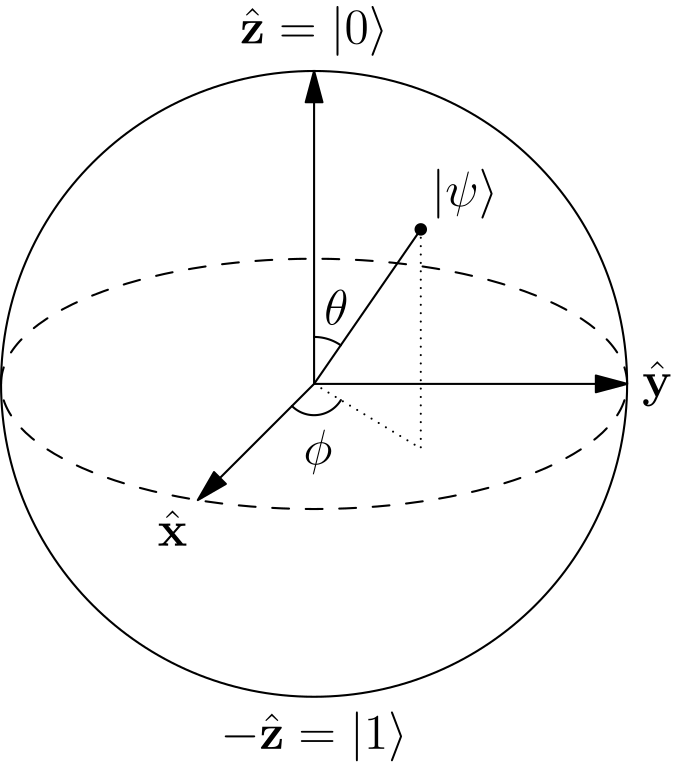
\includegraphics[width=0.4\linewidth]{Figures/677px-Bloch_Sphere.svg}
	\caption{Esfera de Bloch, on es representa un estat arbitrari $\ket{\psi}$ amb els vectors $\hat{\mathbf{x}}, \hat{\mathbf{y}}, \hat{\mathbf{z}}$ representat els eixos ortonormals de la esfera.}
	\label{fig:677px-blochsphere}
\end{figure}

%Glosser.ca, CC BY-SA 3.0 <https://creativecommons.org/licenses/by-sa/3.0>, via Wikimedia Commons
\subsection{Operacions per a només un qubit}
\label{only_one_qubit}
Una vegada es té la informació representada, estaria bé poder operar amb aquella informació, aquest es justament lo que fa que els ordinadors siguin ordinadors, poder operar amb la informació. En computació quàntica els qubits al poder ser representats amb vectors que tenen els seus coeficients són operats per les anomenades portes lògiques quàntiques, que són matrius. Per exemple, si es vol passar de tindre un qubit en l'estat $\ket{0}$ al estat $\ket{1}$, s'utilitza la porta lògica $X$ representada a continuació:
$$
X = \begin{bmatrix}
	0 & 1\\
	1 & 0\\
\end{bmatrix}
$$ 
Podem veure com fa l'acció al multiplicar la matriu per el vector: 
$$
\begin{bmatrix} 0 & 1\\ 1 & 0\\ \end{bmatrix} \begin{bmatrix}1 \\ 0 \end{bmatrix} = \begin{bmatrix}0 \\ 1 \end{bmatrix}
$$
Que en notació de Dirac s'expressaria com: 
$$
X\ket{0} = \ket{1}
$$
D'una manera més general: 
$$
\begin{bmatrix} 0 & 1\\ 1 & 0\\ \end{bmatrix} \begin{bmatrix}\alpha \\ \beta \end{bmatrix} =
\begin{bmatrix} 0\times\alpha & 1\times\beta \\
	1\times\alpha & 0\times\beta \\
\end{bmatrix}
= \begin{bmatrix} \beta \\ \alpha \end{bmatrix}
$$
Es pot veure que aquesta matriu lo que fa és donar la volta als coeficients d'un vector, per tant:
$$
X\ket{0} = \ket{1} \text{ i } X\ket{1} = \ket{0}
$$

Aquesta porta lògica forma part d'un grup important, les matrius de Pauli. Hi han 3 d'aquestes la X, la Y i la Z, usualment representades per $X$, $Y$, $Z$ o per $\sigma_x, \sigma_y, \sigma_z$. Aquestes matrius són les següents:
$$
	 X = \begin{bmatrix} 0 & 1\\ 1 & 0\\ \end{bmatrix} \; Y = \begin{bmatrix} 0 & i\\ -i & 0\\ \end{bmatrix} \; Z = \begin{bmatrix} 1 & 0\\ 0 & -1\\ \end{bmatrix} 
$$

Aquestes matrius són molt important en la mecànica quàntica\footnote{Al ser Hermitianes són observables, concretament ho són dels que corresponen al spin d'una partícula amb spin $\frac{1}{2}$ bàsicament estan relacionades amb els operadors del moment angular.} i són utilitzades àmpliament per descompondre i com a portes lògiques quàntiques.

A partir d'elles podem elaborar matrius que facin una rotació de qualsevol angle  en un del eixos de la representació geomètrica d'un qubit \ref{fig:677px-blochsphere}: 
\begin{align}
	& R_x(\theta) =  e^{-i\theta X/2} = \cos \frac{\theta}{2}I -i \sin \frac{\theta}{2}X = 
	\begin{bmatrix}
		\cos \frac{\theta}{2} & -i \sin \frac{\theta}{2} \\
		-i\sin \frac{\theta}{2} & \cos\frac{\theta}{2} \\
	\end{bmatrix} \label{eq:rx}\\
	& R_y(\theta) =  e^{-i\theta Y/2} = \cos \frac{\theta}{2}I -i \sin \frac{\theta}{2}Y = 
	\begin{bmatrix}
		\cos \frac{\theta}{2} & -\sin \frac{\theta}{2} \\
		\sin \frac{\theta}{2} & \cos\frac{\theta}{2} \\
	\end{bmatrix} \label{eq:ry}\\
	& R_y(\theta) =  e^{-i\theta Z/2} = \cos \frac{\theta}{2}I -i \sin \frac{\theta}{2}Z = 
	\begin{bmatrix}
		e^{-i\theta/2} & 0 \\
		0 & e^{i\theta/2} \\
	\end{bmatrix} \label{eq:rz}
\end{align}
Per exemple la matriu $R_y(\cdot)$ (Eq.\ref{eq:ry}) correspon a una rotació en el eix $\hat{\mathbf{y}}$ de la esfera de la figura \ref{fig:677px-blochsphere}. 
%The quantity of information that a qubit has is the information of all possible combination that the qubit has. One qubit has two possible combination $\ket{0}$ and $\ket{1}$, meanwhile two qubits have four possible combinations $\ket{00}, \ket{01}, \ket{10}, \ket{11}$, and four qubits have $2^4$ possible combinations, that is a total of $16$. And the information about each combination is a complex number, represent in the examples above has $\alpha_i$. The complex numbers are used to specify the quantum superposition that the system has. 

Aquestes operacions poden resultar en superposicions si es fan rotacions amb certs angles. Però hi ha una porta lògica especial per poder fer una rotació que resulta en una superposició uniforme. Es a dir una superposició que tingui les mateixes probabilitats de resultar en $\ket{0}$ o $\ket{1}$\footnote{Un 50\% cada una.}. Aquesta és la porta de Hadamard, denotada per $H$:
\begin{equation}
	H = \frac{1}{\sqrt{2}}\begin{bmatrix}
		1 & 1 \\ 1 & -1
	\end{bmatrix}
\end{equation}
Podem comprovar que és una superposició uniforme al aplicar-la al estat $\ket{0}$:
$$
H\ket{0} = \frac{1}{\sqrt{2}}\begin{bmatrix}1 & 1 \\ 1 & -1 \end{bmatrix}\begin{bmatrix}1 \\ 0\end{bmatrix} = \begin{bmatrix} \frac{1}{\sqrt{2}} \\ \frac{1}{\sqrt{2}} \end{bmatrix}
$$
L'estat resultant és un estat especial que s'escriu com $\ket{+}$\footnote{Un altre estat similar és $\frac{\ket{0} - \ket{1}}{\sqrt{2}}$, quan la matriu $H$ s'aplica al estat $\ket{1}$.} La probabilitat de que un estat col·lapsi en una determinada base és el coeficient de la seva base elevat al quadrat. Com que l'estat és:
$$
\ket{+} = \begin{bmatrix} \frac{1}{\sqrt{2}} \\ \frac{1}{\sqrt{2}} \end{bmatrix} = \frac{\ket{0} + \ket{1}}{\sqrt{2}} =  \frac{1}{\sqrt{2}}\ket{0} +  \frac{1}{\sqrt{2}}\ket{1}
$$
Al elevar al quadrat qualsevol del coeficients es pot veure que dona $\frac{1}{2}$:
$$
\left(\frac{1}{\sqrt{2}}\right)^2 = \frac{1}{2}
$$
Llavors tenim que la probabilitat per obtindre ambos estats és la mateixa, es a dir que si mesurem l'estat $\ket{+}$ hi ha la mateixa probabilitat de que surti $\ket{0}$ o $\ket{1}$. La porta lògica de Hadamard és molt important ja que s'utilitza per crear distribucions uniformes, ja sigui en un qubit o en diversos \footnote{S'aplica aquesta operació a cada qubit del sistema.}.

Altres operacions importants de només un qubit són les portes $S$ i $T$:
$$
S=\begin{bmatrix} 1 & 0 \\ 0 & 1 \end{bmatrix} \; T=\begin{bmatrix} 1 & 0 \\ 0 & e^{i\pi/4} \end{bmatrix}
$$


\subsection{Circuit quàntics}
Aquestes operacions usualment es representen a través de circuits quàntics. Són representacions gràfiques que indiquen de quines operacions s'apliquen a quins qubits i en quin ordre\footnote{A mi em semblen semblats a les partitures musicals.}. 

La forma de representar una porta $H$ aplica a un qubit és amb el circuit quàntic:
\begin{center}
	\begin{quantikz}
		\lstick{$\ket{0}$} & \gate{H} & \qw
	\end{quantikz}
\end{center}

El qubit es representat per la línea que comença amb $\ket{0}$, amb $\ket{0}$ sent el seu estat inicial. Aquests diagrames es llegeixen d'esquerra a dreta, la mateixa forma en la qual s'apliquen les operacions. 

Un qubit en el qual se li aplica una porta $H$ i després una porta $X$, es representat com:
\begin{center}
	\begin{quantikz}
		\lstick{$\ket{0}$} & \gate{H} & \gate{X} & \qw
	\end{quantikz}
\end{center}

Múltiples qubits son simplement més línies, aquí estan representat dos qubits amb portes $X$ aplicades a cada un: 
\begin{center}
	\begin{quantikz}
		\lstick{$\ket{0}$} & \gate{X} & \qw \\
		\lstick{$\ket{0}$} & \gate{X} & \qw 
	\end{quantikz}
\end{center}

Amb múltiples qubits també hi han un ordre en el qual les portes s'han d'aplicar, un circuit en el qual es representa que s'aplica una porta Hadamard al primer, al principi, i una rotació\footnote{D'un angle $\theta$.} en l'eix $x$ en el segon qubit a continuació, seria:
\begin{center}
	\begin{quantikz}
		\lstick{$\ket{0}$} & \gate{H} & \qw& \qw \\
		\lstick{$\ket{0}$} & \qw & \gate{R_x(\theta)} & \qw
	\end{quantikz}
\end{center}



\subsection{Operacions per a múltiples qubits}
Lo realment interessant es quan s'apliquen portes a diversos qubits, perquè d'aquesta manera és pot arribar a tindre qubits entrellaçats. La porta més útil per entrellaçar qubits és la $\mathrm{CNOT}$ o \textit{Controlled NOT}:
\begin{equation}
	\mathrm{CNOT} = 
	\begin{bmatrix}
		1 & 0 & 0 & 0 \\
		0 & 1 & 0 & 0 \\
		0 & 0 & 0 & 1 \\
		0 & 0 & 1 & 0 \\
	\end{bmatrix}
\end{equation}

És bàsicament una porta $X$\footnote{També anomenada porta $\mathrm{NOT}$ degut al paral·lelisme que es fa amb la porta lògica del ordinadors clàssics NOT \cite{wiki:NOT_gate} que simplement inverteix els bits d'1 a 0 (i viceversa), igual que $X$ que inverteix els qubits $\ket{1}$ a $\ket{0}$ i viceversa.} que està controlada per un altre qubit, si l'altre qubit és $\ket{1}$ s'aplica la porta $X$ al altre qubit. Però si l'altre qubit està en superposició, per exemple en $\ket{+}$, aquesta superposició es passa també al qubit controlat, i al mesurar el qubit, la probabilitat de que s'apliqui la porta $X$ és la probabilitat de mesurar l'estat $\ket{1}$. Es considera que aquests qubits estan entrellaçats, una mesura a un d'ells afecta a la mesura del altre. El qubit al qual se li aplica la porta $X$ es diu \textit{target} i el qubit sobre el qual depèn el \textit{target} és el \textit{control}. 

Aquesta porta representa en un circuit s'escriu com:
\begin{center}
	\begin{quantikz}
		& \ctrl{1} & \qw \\
		& \targ{} & \qw
	\end{quantikz}
\end{center}
On el qubit \textit{control} és el primer i on el segon és el \textit{target}, el qubit que té el símbol $\oplus$\footnote{A vegades escriure els circuits quàntics sense especificar l'estat inicial degut a que no és necessari.}. 


\subsubsection{Entrellaçament quàntic}
L'exemple més senzill d'un entrellaçament quàntic en la computació quàntica son els parells de Bell, que es creen al aplicar a dos qubits una porta $H$ al primer i després una porta $\mathrm{CNOT}$ als dos creant l'estat:
$$
\frac{\ket{00}+\ket{11}}{\sqrt{2}} = \frac{1}{\sqrt{2}}\ket{00} + \frac{1}{\sqrt{2}}\ket{11}
$$
Es pot veure que només hi han dos estats possibles $\ket{00}$ i $\ket{11}$ que tenen la mateixa probabilitat associada\footnote{Això es pot veure al elevar al quadrat els coeficients del dos, que donen $\frac{1}{2}$.}. S'afecten l'un al altre en el sentit que quan es mesura només un dels qubits i dona per exemple $\ket{1}$, al mesurar l'altre també dona $\ket{1}$, d'aquesta manera acabant amb l'estat $\ket{11}$. En altres paraules, la mesura d'una part del sistema determina el resultat d'una mesura en una altre part del sistema.

Matemàticament un sistema quàntic, e.i. un conjunt de qubits, està entrellaçant quan aquest sistema no es pot descriure amb un producte tensorial de les parts. Per exemple estat $\ket{00}$ es pot escriure com $\ket{0}\otimes\ket{0}$, mentre que l'estat $\frac{\ket{00} + \ket{11}}{\sqrt{2}}$, no. Per tant el primer no és sistema amb qubits entrellaçats i el segon si ho és.

A partir del entrellaçament i la superposició és com els ordinadors quàntics arribem a tenir avantatges en complexitat sobre els ordinadors clàssics, per més informació sobre els avantatges que presenten els algoritmes quàntics en certes tasques veure l'apèndix \ref{complexity}. 

\subsubsection{Operacions controlades}
A part de la porta $\mathrm{CNOT}$ existeixen diverses portes quàntiques controlades. Realment és pot controlar qualsevol porta, en altres paraules, si l'estat del qubit \textit{control} és $\ket{0}$, s'aplica qualsevol porta al qubit \textit{target}. Fins i tot podem haver-hi diversos qubits \textit{control} i \textit{target}. 

Per exemple existeix la porta Toffoli\footnote{Inventada per Tommaso Toffoli XD}:
\begin{center}
	\begin{quantikz}
		& \ctrl{1} & \qw \\
		& \ctrl{1} & \qw \\
		& \targ{} & \qw
	\end{quantikz}
\end{center}
Que en la seva forma matricial és:
$$
\begin{bmatrix}
	1 & 0 & 0 & 0 & 0 & 0 & 0 & 0 \\
	0 & 1 & 0 & 0 & 0 & 0 & 0 & 0 \\
	0 & 0 & 1 & 0 & 0 & 0 & 0 & 0 \\
	0 & 0 & 0 & 1 & 0 & 0 & 0 & 0 \\
	0 & 0 & 0 & 0 & 1 & 0 & 0 & 0 \\
	0 & 0 & 0 & 0 & 0 & 1 & 0 & 0 \\
	0 & 0 & 0 & 0 & 0 & 0 & 0 & 1 \\
	0 & 0 & 0 & 0 & 0 & 0 & 1 & 0 \\
\end{bmatrix}
$$
Aquesta porta aplica una porta $X$ al últim qubit en cas de que els dos primers siguin $\ket{0}$. 

Tornant a dos qubits, al veure la matriu per la porta $\mathrm{CNOT}$, es pot apreciar que està comporta per una una matriu identitat i una porta $X$\footnote{La matriu identitat es troba a la cantonada superior esquerra, mentre que la porta $X$ es troba al altre extrem.}:
$$
\begin{bmatrix}
	1 & 0 & 0 & 0 \\
	0 & 1 & 0 & 0 \\
	0 & 0 & 0 & 1 \\
	0 & 0 & 1 & 0 \\
\end{bmatrix}
$$
També al veure la porta $Z$ controlada ($\mathrm{CZ}$), es pot apreciar el mateix patró:
$$
\begin{bmatrix}
	1 & 0 & 0 & 0 \\
	0 & 1 & 0 & 0 \\
	0 & 0 & 1 & 0 \\
	0 & 0 & 0 & -1 \\
\end{bmatrix}
$$
Amb la matriu de la porta $Z$ a la cantonada inferior dreta. Aquesta porta en un circuit quàntic es representa de la següent manera:
\begin{center}
	\begin{quantikz}
		& \ctrl{1} & \qw \\
		& \control{} & \qw
	\end{quantikz}
\end{center}

On obstant, una operació controlada de qualsevol unitària $U$ es forma a través del següent circuit: 
\begin{center}
	\begin{quantikz}
		& \ctrl{1} & \qw \\
		& \gate{U} & \qw
	\end{quantikz}
	=
	\begin{quantikz}[align equals at=1.5, column sep=0.3cm]
		& \qw & \ctrl{1} & \qw & \ctrl{1} & \gate{\begin{bmatrix}
				1 & 0 \\
				0 & e^{i\alpha}
		\end{bmatrix}}\\
		& \gate{C} & \targ{} & \gate{B} & \targ{} & \gate{A}
	\end{quantikz}
\end{center}

On $U, \alpha, A, B$ i $C$ son tals que $U = e^{i\alpha}AXBXC$ i  $ABC = I$.

\section{Mesurament quàntic}
Com ja s'ha esmentat a la secció \ref{only_one_qubit} al elevar al quadrat el coeficient d'un estat base que forma part d'un estat, s'obté la probabilitat d'obtenir l'estat base quan es mesura. 

Aquesta és la forma més simple de poder predir el mesurament d'un estat quàntic. Però hi han més coses a dir que son útils. 

Els mesuraments quàntics són un conjunt d'operadors de mesura ${M_m}$, la probabilitat del estat $m$ associat a un operador $M_m$, és:
\begin{equation}
	\mathrm{prob}(m)=\bra{\psi}M_{m}^\dagger M_{m}\ket{\psi}
\end{equation}
\label{eq:Mm}
On l'estat després de la mesura, és:
$$
\frac{M_{m}\ket{\psi}}{\sqrt{\bra{\psi}M_{m}^\dagger M_{m} \ket{\psi}}}
$$
Els operadors ${M_m}$ han de complir que las suma de les seves probabilitats sigui u:
$$
1 = \sum_m \mathrm{prob}(m) = \sum_m \bra{\psi}M_{m}^\dagger M_{m}\ket{\psi}
$$

La diferencia entre aquesta manera de fer les mesures i elevar els coeficients al quadrat, és que l'equació \ref{eq:Mm} és una forma més general, on en comptes de mesurar en la base computacional, és pot mesurar en qualsevol base. A més a més, utilitzant aquest mètode no es necessari saber la composició\footnote{Els coeficients del estats base que descomponen el vector.} del estat que vols mesurar. 

Per mesurar en la base computacional un \textit{statevector} s'utilitzen operadors de mesura derivats de la base computacional amb productes exteriors. Per crear l'aplicació lienal ${M_i}$ associat a la base computacional $\ket{i}$ s'agafa el producte exterior de la base:
$$
M_i = \ket{i}\bra{i}
$$
Per tant la probabilitat que la mesura del estat $\ket{\psi}$ resulti en $\ket{0}$, és:
$$
\mathrm{prob}(\ket{0} = \bra{\psi}\ket{0}\bra{0}^\dagger \ket{0}\bra{0}\ket{\psi}
$$
Per $\ket{\psi} = \ket{0}$ tenim que\footnote{Cal notar que $\ket{0}\bra{0}^\dagger =) \ket{0}\bra{0}$ i que $\ket{0}$ és un vector unitari.}:
\begin{align*}
	\mathrm{prob}(\ket{0}) &= \bra{0}\ket{0}\bra{0}^\dagger \ket{0}\bra{0}\ket{0} \\
	&= \bra{0}\ket{0}\bra{0} \ket{0}\bra{0}\ket{0} \\
	&= \bra{0}\ket{0}\bra{0}\ket{0} \\
	&= 1
\end{align*}
El resultat té sentit degut a que si mesurem $\ket{0}$ en la base $\ket{0}$, esperem que el resultat sigui $1$. 

\section{Matriu de densitat}
Una serie de qubits es pot representar tant per un vector com per una matriu, anomenats \textit{statevector} i \textit{density matrix}, respectivament \cite{QCandQI}.
En aquesta secció aniré ràpidament sobre el concepte de la matriu de densitat i com les operacions que s'apliquen a un \textit{statevector} poden ser aplicades a una \textit{density matrix}. Desprès parlaré del mesuraments parcial d'un sistema, un concepte que es important per la part experimental del treball. 

Una matriu densitat és la representació matemàtica d'un estat quàntic a partir de d'un matriu, es a dir, d'un operador. Aquesta representació serveix descriure sistemes quàntics que no són completament coneguts. Concretament aquests operadors són conjunts de estats quàntics, per un sistema que es descriu amb el estats $\ket{\psi_i}$ que tenen probabilitats $p_i$\footnote{$i$ és l'índex que relaciona un estat a un probabilitat.} la matriu densitat del sistema $\rho$ \cite{QCandQI:density_matrix}:
$$
\rho = \sum_i p_i\ket{\psi_i}\bra{\psi_i}
$$
Cal matriu densitat pot ser simplement $\ket{\psi}\bra{\psi}$ per un estat qualsevol $\ket{\psi}$, per exemple la matriu que representa $\ket{0}$ és:
$$
\rho = \ket{0}\bra{0} = \begin{bmatrix}
	1 & 0 \\
	0 & 0 
\end{bmatrix}
$$

L'evolució d'un estat $\rho$ que descriu un sistema quàntic, al igual que amb els vectors, s'efectua a partir d'operadors unitaris\footnote{Recorda que han de preservar la norma del vector, i en el cas de les matrius la seva traça.}, d'aquesta manera tenim que la evolució d'un operador densitat és:
$$
\sum_i p_i U \ket{\psi_i}\bra{\psi_i} U^\dagger = U\rho U^\dagger 
$$

Al igual que es fan mesures en \textit{statevectors}, les podem amb les \textit{density matrices}. Per operadors de mesura $M_m$, tenim que la probabilitat de tindre l'estat $m$ és:
\begin{align*}
	\mathrm{prob}(m) &= \bra{\psi_i}M_m^\dagger M_m\ket{\psi_i} = \tr(M_m^\dagger M_m \ket{\psi_i}\bra{\psi_i})\\ &= \tr(M_m^\dagger M_m \rho)
\end{align*}
També tenim que l'estat $\ket{\psi_i}$ després de la mesura $m$ és \cite{QCandQI:density_matrix}:
\begin{equation}
	\ket{\psi_i} = \frac{M_m\ket{\psi_i}}{\sqrt{\bra{\psi_i}M_m^\dagger M_m \ket{\psi_i}}} = \frac{M_m\ket{\psi_i}}{\sqrt{\tr(M_m^\dagger M_m \rho)}}
	\label{eq:post_state_rho}
\end{equation}

La equació \ref{eq:post_state_rho} es pot reescriure en termes d'una matriu de densitat després d'una mesura:
\begin{align*}
	\rho_m &= \sum_i p_i \frac{M_m\ket{\psi_i}\bra{\psi_i}M_m^\dagger}{\tr(M_m^\dagger M_m \rho)} \\
	&= \frac{M_m\rho M_m^\dagger }{\tr(M_m^\dagger M_m\rho)}
\end{align*}
Perquè això sigui cert els operadors de mesura $M_m$, ha'n de satisfer: 
$$
\sum_m M_m^\dagger M_m = I
$$
Per a tots els estats possibles $m$.

Per últim s'ha de recordar que les matrius densitat al igual que els vectors d'estat han de tenir certes característiques: 
\begin{enumerate}
	\item La traça de $\rho$ ha d'equivaler $1$.
	\item $\rho$ ha de ser un operador positiu\footnote{Un operador positiu $A$ es aquell que $\bra{\psi}A\ket{\psi}\geq0, \forall \ket{\psi}$.}.
\end{enumerate}
\subsection{Matriu de densitat reduïda}
Una aplicació important dels operadors de densitat és la descripció d'estats parcials amb el operador de densitat reduït, i per tant la descripció dels mesuraments parcials. 

Al tindre un sistema físic compost de dos sistemes $A$ i $B$ que es descriu per una matriu de densitat $\rho^{AB}$, la matriu de densitat reduït del sistema $A$ és:
\begin{equation}
\rho^A = \tr_B(\rho^{AB})
	\label{eq:partial_trace}
\end{equation}
On $\tr_B$ és la traça parcial sobre el sistema $B$, que es defineix per l'equació següent \cite{QCandQI:partial_trace}: 
\begin{equation*}
	\tr_B(\ket{a_1}\bra{a_2}\otimes\ket{b_1}\bra{b_2}) = \ket{a_1}\bra{a_2}\tr(\ket{b_1}\bra{b_2})
\end{equation*}
Amb $\ket{a_1}$ i $\bra{a_2}$ sent estats vàlid pel sistema $A$, i $\ket{b_1}$ i $\bra{b_2}$ sent-ho per $B$. El terme $\tr(\ket{b_1}\bra{b_2})$ s'omet quan els els vectors del producte exterior son iguals i formen un operador de densitat vàlid, el qual la traça ha de donar $1$.

No obstant aquesta definició no es pot utilitzar quan no saps com representar la matriu de densitat $\rho$ com a un producte vectorial, en el qual un dels termes és l'estat que es traça afora. En altres paraules, en la equació \ref{eq:partial_trace} si no es coneix $\rho^A$ i $\rho^B$ per $\rho^{AB} = \rho^A\otimes\rho^B$, aquesta equació no serveix de res.  

Degut a això en el llibre de text \textit{Quantum Computing: A Gentle Introduction} \cite{QC_intro} els autors defineixen la traça parcial d'una altre manera més general, on només s'ha de saber les bases del sistemes $A$ i $B$ i un operador vàlid per el sistema $AB$. Per una matriu de densitat $\rho^{AB}$ que representa el sistema $A\otimes B$, la traça parcial de $\rho^{AB}$ sobre $B$ és:
$$
\tr_B \rho^{AB} = \sum_i \bra{\beta_i}\rho^{AB}\ket{\beta_i}
$$
On el conjunt ${\beta_i}$ són les bases del sistema $B$. Les entrades de la matriu $\tr_B \rho^{AB}$ representades en termes de les bases ${\ket{\alpha_i}}$ i ${\ket{\beta_j}} $del sistemes $A$ i $B$ respectivament, són:
$$
(\tr\rho^{AB})_{ij} = \sum_{k=0}^{M-1} \bra{a_i}\bra{\beta_k}\rho^{AB}\ket{\alpha_j}\ket{\beta_k}
$$
Amb la matriu sent:
$$
\tr\rho^{AB} = 
\sum_{i,j=0}^{N-1}\left(\sum_{k=0}^{M-1} \bra{a_i}\bra{\beta_k}\rho^{AB}\ket{\alpha_j}\ket{\beta_k}\right) \ket{\alpha_i}\bra{\alpha_j}
$$
On $N$ és la dimensió del sistema $A$ i $M$ és la dimensió del sistema $B$. 

Es pot comprovar que aquestes definicions són correctes degut a que en els dos llibres utilitzen les seves definicions per tractar el mateix cas i obtenen el mateix resultat \cite{QCandQI:example_partial, QC_intro:example_partial}.

\subsubsection{Mesurament parcial}
\label{par_measurament}
Es pot arribar a treure una mesura parcial sobre un sistema de qubits amb la traça parcial i operadors de mesura. En el paper fet per Huang et.al. \cite{QGAN_exp} es descriu un estat $\rho$ després d'un mesurament parcial $\Pi_A$ sobre un sistema $A$ del estat $\ket{\psi}$ com:
$$
\rho = \frac{\tr_A(\Pi_A \ket{\psi}\bra{\psi})}{\tr(\Pi_A\otimes I_{2^N-2^{N_A}}\ket{\psi}\bra{\psi})}
$$
El sistema $A$ està compost per $N_A$ qubits per tant la resta del estat $\ket{\psi}$ té $N-N_A$, on $N$ és el nombre total de qubits del estat $\ket{\psi}$. D'aquesta manera $\Pi_A\otimes I_{2^N-2^{N_A}}$ té $2^N\times 2^N$ dimensions i pot ser multiplicat per la matriu $\ket{\psi}\bra{\psi}$ que té les mateixes dimensions. No obstant sorgeix un problema amb el numerador de l'equació perquè $\Pi_A$ no té les mateixes dimensions que $\ket{\psi}\bra{\psi}$, encara no he pogut utilitzar aquesta equació adequadament. No sé com computar-la. Parlaré d'això més endavant en la part experimental d'aquest treball.

En el mateix paper es planteja la mateixa equació però per l'estat post-mesura expressat en forma de vector d'estat, molt semblat a l'equació \ref{eq:post_state_rho}. L'única diferencia es que en l'equació del paper no s'expressa el operador de mesura en la forma $M_m^\dagger M_m$, en canvi el autors ho expressen tan sols com $\Pi_A$, més concretament  $I_{2^N-2^{N_A}}\otimes \Pi_A$. Potser la forma plantejada per els autors té en compte el conjugat hermitià, però no estic segur.
L'equació esmentada en l'article és la següent:
$$
\ket{\psi_m} = \frac{I_{2^N-2^{N_A}}\otimes\Pi_A\ket{\psi}}{\sqrt{\tr(I_{2^N-2^{N_A}}\otimes\Pi_A\ket{\psi}\bra{\psi})}}
$$
Al igual que l'equació per les matrius de densitat parlaré d'aquesta contradicció en la part experimental.

\section{Ordinadors quàntics}
Tota aquesta teoria és aplicada a través de qubits físics que s'ubiquen al ordenadors quàntics. Hi han diversos tipus d'ordinadors quàntics, degut a que els qubits poden ser diversos sistemes. Poden ser fotons, chips de silici superconductors o ions atrapats per imants. No elaboraré més sobre aquest tema degut a que no és el tema central d'aquest treball, m'he centrat molt més en la teoria. 

Però si vull generar imatges amb un ordinador quàntic, no necessito un? No, perquè puc simular l'evolució dels estats quàntics amb un ordinador, pensa que tot ser expressat amb àlgebra lienal. No obstant, quan s'intenta simular un sistema quàntic de molt qubits\footnote{Més de 50 per exemple.} un ordinador de sobretaula tardaria molt de temps i realment no és viable. Per més informació sobre algoritmes quàntics i com s'executen en ordinadors i en simuladors, es pot llegir l'apèndix \ref{complexity}.  


\chapter{Intel·ligència artificial}

Segurament has sentit parlar de l'intel·ligènica artificial o de les xarxes neuronals, són conceptes que semblen abstractes però jo penso que son bastant intuïtius, intentaré que tú et sentis de la mateixa manera al final d'aquest capítol. 

Intel·ligència artificial és un mot una mica ambigu, que és refereix a qualsevol algoritme que entra dintre del camps del \textit{machine learning} o aprenentatge automàtic\footnote{No obstant, col·loquialment s'utilitza per denominar a qualsevol algoritme o robot que és intel·ligent o sembla que és intel·ligent. }. Aquests algoritmes simplement s'alteren a ells mateixos per fer millor la tasca que s'ha li ha designat, no importa quin és el objectiu o com ho aconseguix, lo que importa és si aprèn automàticament. Cal notar que els canvis que s'efectuen sobre si mateixos no han de ser predeterminats, si l'algoritme té una llista de les instruccions que va executant segon la situació no seria ven bé una intel·ligència o un algoritme de \textit{machine learning}. 

La manera que tenen aquests algoritmes d'alterar-se a si mateixos usualment es canviant els paràmetres de les operacions dels quals estan compostos. Per exemple, en una regressió lineal, s'actualitzen els paràmetres de la recta que representa la tendència de les dades, com es pot veure a la figura ref{fig:leastsquares}.

\begin{figure}
	\centering
	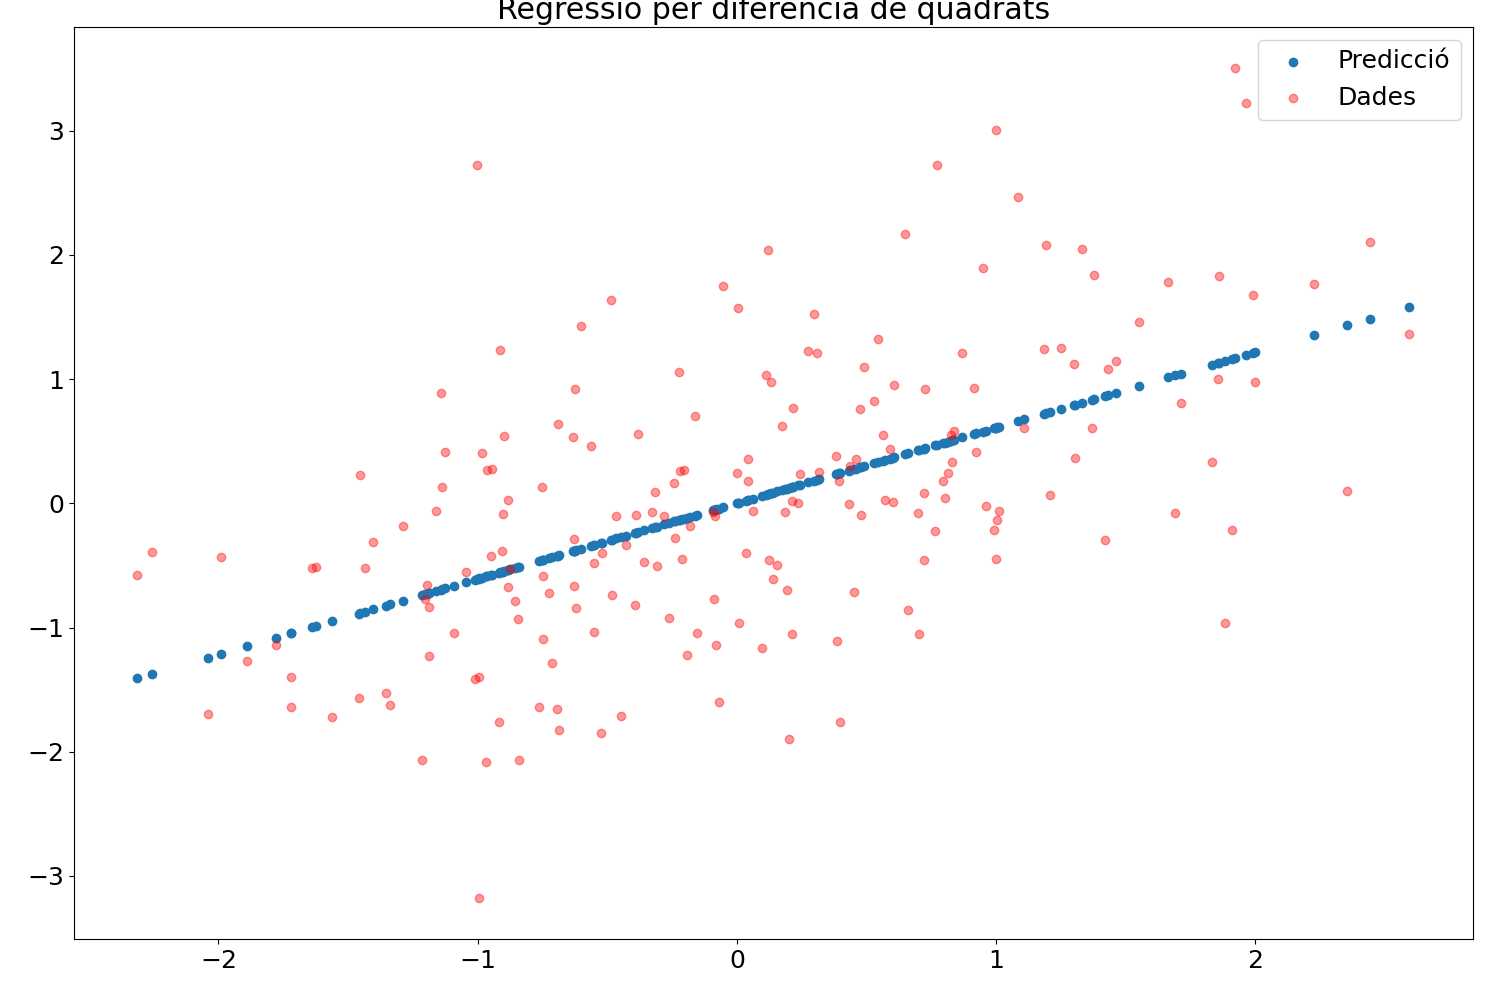
\includegraphics[width=0.7\linewidth]{Figures/least_squares}
	\caption{Exemple d'una regressió lineal de dades generades al atzar. Veure el codi a \ref{lst:linear_regression}.}
	\label{fig:leastsquares}
\end{figure}

Hi han diversos mètodes per ajustar els paràmetres, el més comú es ajustar-los segons la derivada d'una funció anomenada funció de pèrdua o \textit{loss function}, usualment representada per la lletra $\mathcal{L}$. Aquesta funció representa els objectius del programa i pot ser minimitzada o maximitzada, per exemple, en una regressió lienal es vol reduir la distancia entre els \textit{data points} o dades i la línia que prediu la tendència, Fig. \ref{fig:leastsquares}. 

Degut a que es poden realitzar molts tipus de funcions de pèrdua, ja sigui per la forma de la funció en si o per els paràmetres de la funció. Per conseqüència, el programes de \textit{machine learning} són extremadament versàtils, la màxima expressió d'això es pot veure en les xarxes neuronals o \textit{neural networks}. Aquests algoritmes són els més potents, complexos i polivalents. Precisament utilitzo un d'aquests per generar les imatges. Són àmpliament utilitzats pel reconeixement d'imatges, traducció i sintetització de textos, conducció automàtica, algoritmes de recomanació i es clar, generació d'imatges \tocite. 

\section{Xarxes neuronals}
Aquests tipus d'algoritmes que entren dintre de la categoria de \textit{machine learning} no tenen un nombre que fa recordar a les xarxes de neuronals que formen part del nostre sistema nerviós central per casualitat, estan directament inspirades en els nostres cervells. Són uns programes que consisteixen en la connexió de diverses operacions anomenades neurones, que conjuntament formen una xarxa, la qual s'organitza a partir de capes. Segons la variació del tipus de neurona i la estructura que aquestes formen podem tindre algoritmes destinats a fer diferents tasques. Això juntament amb els diversos tipus de funció de pèrdua contribueix a la versatilitat de les xarxes neuronals. Aquests models d'intel·ligencia artificial constitueixen el camp del \textit{deep learning} o aprenentatge profund. S'anomenen d'aquesta forma per referenciar la profunditat d'aquests algoritmes, es a dir el nombre de capes que tenen.

Una neurona consisteix simplement en una suma ponderada, una altra suma i una funció no lineal que s'aplica al resultat. Les neurones tenen com input i output vectors. Per tant, una neurona es pot definit com:
$$
\sigma \left(\sum_{i=1}^n w_i x_i + b\right) = \sigma \left( w_1x_1 + w_2x_2 + \cdots + w_nx_n + b 
\right) 
$$
Per $\sigma$ sent una funció no lienal i $n$ sent la mida del vector. Després estan el paràmetres, $w_i$ i $b$, anomenats \textit{weights} i \textit{bias}. 
Aquests paràmetres tenen una utilitat pot clara, per això tenim que parlar en termes d'importància. En altres paraules, com afecta cada paràmetre a una part de la xarxa i també com afecta aquest al output de la xarxa. Després de deixar clara l'equació s'ha d'il·lustrar la interconnectivitat que tenen les neurones entre si. 

Una neurona pot tindre diversos inputs que venen de diverses neurones, el mateix passa amb els outputs. Depèn de com es connectin entre si o de quina operació addicional fan les neurones, aquestes formen diversos tipus de capes. A partir de les tipus de capes i el nombre d'aquestes es com s'especifica l'arquitectura d'una xarxa neuronal. Tornant a l'utilitat del paràmetres, un \textit{weight} especifica com de forta es la relació entre una neurona en una capa i una altre neurona en una capa veïna. I un \textit{bias} especifica com d'important és una neurona, degut a que aquest número afecta al resultat de la suma de la neurona, fent que aquesta sigui més alta.

Usualment l'arquitectura es divideix en tres parts la capa d'input, les capes ocultes i la capa d'output. La quantitat de neurones que hi han a la capa d'inputs es la que defineix la mida del vector que es dona com input a la xarxa, degut a que cada element del vector es dona a cada neurona amb la capa. El mateix passa amb la capa d'outputs, cada output de cada neurona de la capa acaba sent un element en el vector que surt de la xarxa. Per tant el número de neurones que té cadascuna d'aquestes dues capes, especifica la mida del vectors d'input i d'output de la xarxa respectivament. Per exemple si es vol donar com input a una xarxa una imatge de 16 per 16 píxels\footnote{Una imatge en blanc i negre.} calen 256 neurones en la capa d'inputs, una per cada pixel. 

En canvi, les \textit{hidden layers}, es a dir les capes ocultes, no tenen una mida determinades, el mateix passa amb el nombre d'aquestes que té la xarxa. Depenen de cada cas, la quantitat de neurones que tenen aquestes capes i també el nombre d'aquestes, varia. Això, juntament amb el diversos tipus de capa és el que dona la versatilitat d'aquests algoritmes, com ja he comentat. 
 
Entre els diferents tipus de capes que ponen tindre les xarxes neuronals, el més comú i simple d'aquestes és una \textit{fully connected layer}, o una capa completament connectada, veure la figura \ref{fig:560px-artificialneuralnetwork}. Les neurones que formen aquesta capa estan connectades a totes les neurones de la capa anterior i així mateix a totes les neurones de la capa següent. La forma que tenen aquestes capes de variar es mitjançant la mida que tenen, es a dir, la quantitat de neurones que tenen. \begin{figure}
	\centering
	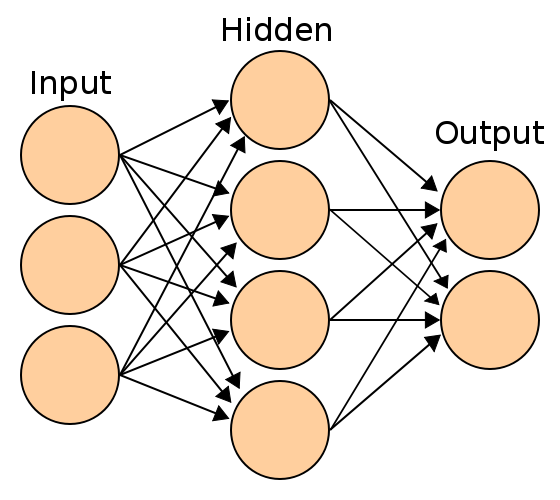
\includegraphics[width=0.7\linewidth]{Figures/560px-Artificial_neural_network.svg}
	\caption{Usualment les xarxes neuronals es representen d'aquesta forma, amb fletxes i boles. Les boles representarien cada neurona i les fletxes mostren com estan connectades. La \textit{hidden layer} d'aquesta representació es pot veure que és una \textit{fully connected layer} degut a com està connectada a les altres capes, rebent cada neurona el output de cada neurona anterior.}
	\label{fig:560px-artificialneuralnetwork}
	% en:User:Cburnett, CC BY-SA 3.0 \href{http://creativecommons.org/licenses/by-sa/3.0/}, via Wikimedia Commons
\end{figure}
També es pot variar la funció d'activació que tenen, que ha de ser una funció no lineal. La més utilitzada és la sigmoide:
$$
f(x) = \frac{1}{1+e^{-1}}
$$

\section{Descens del gradient}
Una vegada he parlar de les xarxes neuronals, he de comentar com aquestes evolucionen al llarg del temps, es a dir com es van actualitzen a si mateixes per complir la tasca que s'ha li's ha encomanat. Ja he comentat que existeix una funció anomenada \textit{loss function}, la qual es deriva per actualitzar els paràmetres de la xarxa. En aquesta secció parlaré més en profunditat d'aquest mecanisme que s'anomena el descens (o ascens) del gradient.

Es comença amb la funció de pèrdua, que esmenta els objectius de la xarxa. Els punts mínims d'aquesta funció representen els punts òptims de la xarxa, els punts als quals es vol arribar. Per exemple, si es volen classificar imatges de gats i gossos, s'assignen dos etiquetes a les imatges, $1$ als gats i $0$ als gossos. Utilitzaré com a exemple la funció de pèrdua \textit{binary cross entropy} o \textit{log Loss} per poder il·lustrar com una funció pot representar si una xarxa neuronal està fent el seu treball o no. La funció \textit{binary cross entropy} és la següent:
\begin{equation}
	\mathcal{L} = - t\log(y) - (1 - t)\log(1 - y) 
	\label{eq:BCE}
\end{equation}
Per $t_i$ sent la etiqueta real que ha de tenir l'imatge i $y_i$ sent la etiqueta que el model dona a l'imatge. Per tant si l'etiqueta real és $1$, l'equació acaba sent:
$$
\mathcal{L}_1 = - \log(y)
$$
I el cas contrari per $t = 0$:
$$
\mathcal{L}_0 = - \log(1 - y)
$$

Si donen com input l'imatge d'un gat i el programa es dona com output $0.92$ tenim que la pèrdua és de:
\begin{align*}
	\mathcal{L} &= - t\log(y) - (1 - t)\log(1 - y) = - \log(0.92) \simeq 0.0834
\end{align*}
En canvi, si el programa es dona un output de $0.15$ la pèrdua seria:
\begin{align*}
	\mathcal{L} &= - t\log(y) - (1 - t)\log(1 - y) = - \log(0.15) \simeq 1.897
\end{align*}
Es pot veure que si l'etiqueta que posa el model s'allunya més de l'etiqueta real la pèrdua és més gran. El mateix es pot veure per les imatges del gossos o en altres paraules les imatges que haurien de tenir etiqueta zero:
\begin{align*}
	\mathcal{L} &= - 0\cdot\log(0.89) - (1 - 0)\cdot\log(1 - 0.89) = - \log(1- 0.89) \simeq 2.207 \\
	\mathcal{L} &= - 0\cdot\log(0.08) - (1 - 0)\cdot\log(1 - 0.08) = - \log(1- 0.08)\simeq 0.0834
\end{align*}
Per tant quan més pròximes estén les prediccions (els outputs del model) a les etiquetes del programa, menor serà la pèrdua, llavors al minimitzar la funció es trobarà el punt òptim on totes les prediccions seran iguals a les etiquetes.

A aquests punts òptims s'han arribat actualitzant els paràmetres a través de la derivada de la funció, concretament a través del gradient. El gradient d'una funció és un vector on els seus elements són la derivada parcial respecte a cada paràmetre (per aclarir, un element per paràmetre). El gradient d'una funció $f(\theta)$ es representa com $\nabla f(\theta)$, i es pot escriure en forma de vector com:
$$
\nabla f(\theta) = \begin{bmatrix}
	\pdv{f}{\theta_1} \\
	\pdv{f}{\theta_2} \\
	\vdots \\
	\pdv{f}{\theta_{n-1}} \\
	\pdv{f}{\theta_{n}}
\end{bmatrix}
$$
No fa falta fixar-se en lo que és exactament un gradient, l'únic que importa es que cada paràmetre de la xarxa neuronal\footnote{Cada \textit{weight} i cada \textit{bias}.} s'ha d'actualitzar acorde amb la derivada. Això es pot entendre com canviar lleugerament un paràmetre acord amb la direcció. Aquesta direcció es indica per la derivada. L'objecte que s'encarrega d'actualitzar-los, s'anomena optimitzador. L'optimitzador més senzill que hi ha és:
$$
\theta_{i}^t = \theta_{i}^{t-1} \pm \eta\pdv{\mathcal{L}(\theta)}{\theta_{i}^{t-1}}
$$
Aquí s'actualitza un paràmetre $\theta_i$, he posat el superíndex $t$ per expressar que s'actualitza, passant d'un temps $t-1$ a $t$. En aquesta equació utilitzo $\theta$ per expressar tots els paràmetres del model. En els optimitzadors s'afegeix un número $\eta$ anomenat \textit{learning rate}. Usualment és un número que petit\footnote{Entre $0.1$ i $0.001$ per exemple.}, aquest paràmetre especifica com de ràpid cabien els paràmetres. El \textit{learning rate} es pot anar ajustant depenen de la situació, del model en el qual s'implementi. Alteracions en aquest pot causar diversos fenòmens tan negatius com positius. Cal notar que en l'optimitzador he utilitzar el signe $\pm$ perquè si és positiu significa que s'està ascendint pel gradient, i si és negatiu s'està descendint. No obstant, usualment s'utilitza el signe negatiu per convenció. 

Al fer la derivada de la funció de pèrdua es pot veure immediatament que s'ha d'aplicar la regla de la cadena, ja que s'ha de fer la derivada del output de la xarxa neuronal degut a que depèn del paràmetre. Al ser les xarxes neuronals funcions molt complexes, s'utilitza una tècnica concreta per efectuar la derivada de la xarxa neuronal anomenada \textit{backpropagation}. 

\subsection{Backpropagation}
Al aplicar la regla de la cadena 'de fora cap a dins' s'ha de començar a derivar per l'última capa i acabar per la primera, d'aquí ve el nom \textit{backpropagation} perquè es propaga l'error en direcció contraria. Mentre que quan es dona un input a xarxa, s'anomena {forward propagation} o \textit{forward pass}.  

No entraré en profunditat sobre la \textit{backpropagation} en aquesta secció, només en limitaré a esmentar la manera en la qual es calcula. 

L'activació d'una neurona $j$ en l'última capa $L$ de la xarxa es defineix com: 
$$
a^{L}_j = \sigma\left(\sum_{j=0}^{n_{L- 1}}w^L_{jk} a^{L-1}_k+ b_j^L\right)
$$
On $a^{L-1}_k$ és l'activació d'una neurona $k$ en la capa anterior $L-1$, i on el \textit{weight} $w^L_{jk}$ és el paràmetre que expressa en que mesura es connecta la neurona $j$ a la neurona $k$. Com ja he dit, expressa com de forta és aquesta connexió. Utilitzant aquesta definició ja es poden fer les derivades. La suma es fa al llarg de $n_{L-1}$ que és el nombre de neurones que té la capa $L-1$.

No obstant, convé definir el terme $z_j^L$ per procedir a fer les derivades. Simplement és l'equació d'una neurona però sense la funció d'activació:
$$
z_j^L = \sum_{j=0}^{n_L - 1}w^L_{jk} a^{L-1}_k+ b_j^L
$$
L'objectiu és obtenir la derivada de la \textit{loss function} respecte a un \textit{weight} qualsevol i un \textit{bias} qualsevol. Per tant, s'han obtenir les següents derivades parcials:
$$
\pdv{\mathcal{L}}{w_{jk}^L} \text{ i } \pdv{\mathcal{L}}{b_j^L}
$$
Començaré amb la derivada del \textit{weight}, a aplicar la regla de cadena obtenim que:
\begin{equation}
	\pdv{\mathcal{L}}{w_{jk}^L} = \pdv{z_k^L}{w_{jk}^L}\pdv{a_j^L}{z_j^L}\pdv{\mathcal{L}}{a_j^L}
	\label{eq:chain_neuron}
\end{equation}
L'última derivada, 'la que està més afora' és simplement la derivada de la funció de pèrdua respecte al output de la xarxa. En el cas de la funció de pèrdua \textit{Squared Error}, és\footnote{No aplico la regla de la cadena en aquesta derivació perquè ja es té en compte en l'equació \ref{eq:chain_neuron}}:
$$
\pdv{\mathcal{L}}{a_j^L} =  \pdv{a_j^L} (a_j^L - y)^2 = 2(a_j^L - y)
$$
On $y$ és la predicció desitjada del model. A continuació, la derivada del resultat de la neurona $a_j^L$ respecte a $z_j^L$, que és la derivada la funció d'activació.
$$
\pdv{a_j^L}{z_j^L} = \sigma'(z_j^L)
$$
Per últim tenim la derivada de $z_j^L$ respecte al \textit{weight}:
$$
\pdv{z_j^L}{w_{jk}^L} = a^{L-1}_k
$$
La derivada és la neurona anterior, cal recordar que el \textit{weight} lo que fa es establir la connexió entre dues neurones, les neurones $j$ i $k$. 

Finalment es pot veure que l'equació \ref{eq:chain_neuron} es pot escriure com\footnote{Deixo l'ultima derivada $\pdv{\mathcal{L}}{a_j^L}$ sense reescriure perquè aquest terme pot variar depenent de la funció de pèrdua que s'utilitza.}:
$$
	\pdv{\mathcal{L}}{w_{jk}^L} = \pdv{z_k^L}{w_{jk}^L}\pdv{a_j^L}{z_j^L}\pdv{\mathcal{L}}{a_j^L} = 
	a^{L-1}_k \sigma'(z_j^L)\pdv{\mathcal{L}}{a_j^L}
$$

No obstant falta un detall, la derivada d'una neurona que passa el seu resultat a diverses neurones. Aquesta derivada és:
$$
\pdv{\mathcal{L}}{a_j^{L-1}} = \sum_{j=0}^{n_{L-1}} \pdv{z_j^L}{a_k^{L-1}}\pdv{a_j^L}{z_j^L}\pdv{\mathcal{L}}{a_j^L}
$$
La suma representa que aquesta neurona té un output que es propaga cap a endavant i afecta a les neurones que estan més endavant. 

Amb aquestes derivades ja es pot desenvolupar el vector gradient, en el qual estan totes les derivades de la \textit{loss function} respecte a tots els paràmetres. Concretament, la mitjana d'aquestes derivades, perquè es vol actualitzar els paràmetres per poder minimitzar la pèrdua en totes les dades disponibles. En altres paraules, si es vol que una xarxa reconegui imatges de gats, se li té que ensenyar moltes imatges de gats. Si només se li ensenya una, només aprendrà a reconèixer aquella imatge. 

Tota aquesta teoria es veurà implementada en la part pràctica en forma de codi, degut a que m'he vist amb la necessitat de tenir una xarxa neuronal programada des de zero. Usualment s'utilitzen plataformes com \textit{TensorFlow} \cite{tensorflow2015-whitepaper} o \textit{PyTorch} \cite{pytorch_2019}.

\section{Generative adversial networks}
Com ja he dit hi han molts tipus de xarxes neuronals, no obstant, en aquest treball només em centraré en un tipus en específic, les xarxes generatives adversatives o \textit{generative adversial networks (GAN)} en anglès.

Aquestes xarxes, com el seu nom diu, s'utilitzen per generar dades, usualment s'apliquen a imatges. Es troben al darrera de projectes com \textit{This person does not exist} \cite{styleGAN, this_person_does_not_exist}, una pàgina web que et genera una cara d'una persona que no existeix, degut a que es una cara generada artificialment a partir d'aquest tipus de models.

Aquests tipus de models van ser introduïts per primera vegada al 2014 per Ian Goodfellow \cite{GAN2014}, des de llavors s'han convertit en un dels models de \textit{deep learning} més sòlids i utilitzats. 

Aquests algoritmes consisteixen en dos models (xarxes) diferents, un generador i un discriminador, amb objectius oposats que s'enfrenen entres si. Per aquesta raó tenen la paraula adversatives en el nom. El generador i discriminador es poden entendre com uns falsificador de bitllets i uns policies que els volen atrapar, respectivament. Els policies es tornen millors al seu treball, podent distingir millor entre els bitllets falsificats i els reals. Els falsificadors responen a això millorant les seves tècniques de falsificació, per tant els policies han de millor encara més. Es un cicle en el qual aquestes forces antagonistes es fan millorar l'una al altra. El mateix passa amb el generador i el discriminador. El discriminadors aprèn a distingir entre les imatges reals i les imatges falses que fabrica el generador, mentre que el generador aprèn a enganyar al discriminador. 

Si s'especifiquen bé els objectius de cada model, arribem a \textit{zero sum game}\footnote{Un \textit{zero sum game} es simplement un joc entre dos jugadors en que per guanyar un l'altre ha de perdre e.g. joc d'estirar la corda entre dos equips.} de teoria de joc. La manera en la que es soluciona es al arribar a un equilibri de Nash \cite{QGAN_exp}, on el discriminador no sap diferenciar entre les imatges reals i les falses\footnote{Que el discriminador no sàpiga diferenciar no implica arribar a un equilibri de Nash, aquest concepte es definit d'una altra forma.}.

En el paper original \cite{GAN2014} s'esmenta un pseudocodi per aquests models, que he representat en l'algoritme \ref{alg:GAN}. En aquest és parla de \textit{minibatch} que és simplement un grup d'imatges o de dades, i de soroll que són dades generades aleatòriament i que es poden com input al generador perquè aquest no generi exactament les mateixes imatges cada vegada. El soroll afegeix variació als outputs del generador, però sempre s'intenta en una petita quantitat. 

\begin{algorithm}
	\caption{Pseudocodi per una xarxa generativa adversativa}\label{alg:GAN}
	\begin{algorithmic}
		\For{número de interaccions}
		\For{$k$ pasos}
		\State Treure minibatch de $m$ mostres de soroll $\{z_i, \cdots, z_m\}$ de la distribució de soroll $p_g(z)$
		\State Treure minibatch de $m$ mostres d'exemples $\{x_i, \cdots, x_m\}$ de la distribució d'exemples $p_{\mathrm{data}}(x)$
		\State Actualitzar el discriminador ascendint el seu gradient: 
		$$
		\nabla_\theta \frac{1}{m}\sum_{i=1}^{m}\left[\log D(x_i) + \log(1- D(G(z_i)))\right]
		$$
		\EndFor
		\State Treure minibatch de $m$ mostres de soroll $\{z_i, \cdots, z_m\}$ de la distribució de soroll $p_g(z)$
		\State Actualitzar el generador descendent el seu gradient:
		$$
		\nabla_\theta \frac{1}{m} \sum_{i=1}^{m} \log(1-D(G(z_i)))
		$$
		\EndFor
	\end{algorithmic}

\end{algorithm}

En el pseudocodi es pot veure que primer s'actualitza el discriminadors $k$ vegades i després  el generador una sola vegada. Això és perquè interessa que el discriminador sàpiga distingir les imatges ràpidament, per poder indicar al generador com generar les imatges. Si el discriminador esmenta que unes imatges de gats són imatges de gossos, el generador fabricarà imatges de gossos, perquè ell aprèn a partir del que indica el discriminador.

També és pot veure com és la funció de pèrdua, que en el paper anomenen \textit{minimax loss function} que és la mateixa que la \textit{Binary Cross Entropy}. Es pot veure que en la BCE, quan $t$ és zero, que seria l'etiqueta per les imatges falses del generador dona $\log(1-y)$. En el cas contrari, per $t$ igual a un, que expressa que les imatges són reals dona $\log(y)$.  


\chapter{Generació d'imatges amb un ordinador quàntic}

Investigadors al veure el potencial que tenen els ordinadors quàntics i l'intel·ligència artificial, no es van poder resistir a crear un nou camp d'investigació, el \textit{Quantum Machine Learning (QML)}, o aprenentatge automàtic quàntic. Al igual que les xarxes neuronals són les estrelles dintre del \textit{machine learning}, les xarxes neuronals quàntiques ho són dintre del \textit{quantum machine learning}. Des de que es va començar a investigar aquests algoritmes s'han arribat a implementar diversos tipus de xarxes neuronals en algoritmes quàntics. Principalment pel que fa a la generació i classificació d'imatges i dades.

No obstant aquests algoritmes no són completament quàntics, usualment consisteixen en actualitzar els paràmetres d'un circuit quàntic perquè aquest generi les dades. On les actualitzacions dels paràmetres es calculen amb un ordinador clàssic. Això es veure molt clar quan expliqui la part pràctica del treball. 

Abans de continuar amb el capítol he de dir que existeixen diversos algoritmes dintre del \textit{quantum machine learning}, no tot en la vida són xarxes neuronals. Per exemple, es pot donar a terme classificació de dades mitjançant \textit{support vector machines}\footnote{Classificar dades de dimensions petites en espais vectorials molt grans \cite{QSVM_2019, QSVM_xanadu_2019}.} o amb un anàleg de la regressió lineal \cite{Q_linear_regression_xanadu}. No obstant, en aquest capítol em centraré exclusivament en les xarxes neuronals quàntiques.

\section{Descens del gradient quàntic}
De moment tindre en consideració que una xarxa neuronal quàntica és un circuit quàntic parametritzat, és a dir que simplement té paràmetres. Això juntament amb una funció de pèrdua i dades que corresponen a aquesta es suficient per explicar com s'actualitzen els paràmetres. 

L'objectiu principal es avaluar la derivada respecte amb un paràmetre. Sorprenentment és dona a terme d'una manera més senzilla que amb una xarxa neuronal clàssica. Simplement s'utilitza la definició de la derivada per avaluar-la. S'altera lleugerament un sol paràmetre i es treu la diferencia entre els dos outputs del circuit quàntic. Aquest mètode per avaluar la derivada s'anomena \textit{parameter shift} \cite{tfq, shift_parameter_harrow_2019}. 

Si un circuit quàntic té paràmetres $\theta$ representats per un vector, per un paràmetre $\theta_{i}$, es defineix un vector de pertubació $\Delta_i$ ple de zeros, de igual mida que $\theta$, però que en la posició de $\theta_i$ té un $1$. A partir del vector de pertubació es pot definir la derivada de la funció de pèrdua $\mathcal{L}(\cdot)$ respecte al paràmetre $\theta_{i}$:
$$
\pdv{\theta_i} \mathcal{L}(\theta) = \mathcal{L}(\theta + \tfrac{\pi}{4}\Delta_i) - \mathcal{L}(\theta - \tfrac{\pi}{4}\Delta_i)
$$
Es pot veure que el vector $\theta \pm \frac{\pi}{4}\Delta_i$ és el vector $\theta$ però amb una petita variació en la posició $i$ que es la que correspon al paràmetre $\theta_i$. Amb aquest mètode ja es pot desenvolupar pràcticament qualsevol actualització de paràmetres, aquesta es la part senzilla de les xarxes neuronals quàntiques, la dificultat radica en la forma dels circuits quàntics que les componen.

\section{Circuits quàntics per xarxes neuronals}
L'única  certesa sobre aquests circuits es que han de estar parametritzats. Usualment estan compostos per una gran quantitat de portes rotacionals parametritzades, les quals ja he presentat en les equacions \ref{eq:rx}, \ref{eq:ry} i \ref{eq:rz}. 

El problema que esmenten en els articles sobre xarxes neuronals quàntiques es que s'han d'implementar funcions no lienals en els circuits, degut a que la complexitat de les xarxes neuronals radica en aquest tipus de funcions. A primera vista por semblar una tasca quasi impossible a causa de la naturalesa lienal de la computació quàntica. No obstant, durant els anys s'han desenvolupat diverses tècniques per donar a terme aquesta fita. 

A partir d'una combinació de rotacions i portes que entrellacen qubits es pot arribar a implementar una funció semblant a la tangent hiperbòlica\footnote{La tangent hiperbòlica també s'utilitza com a funció no-lienal en el \textit{deep learning}.} en un circuit quàntic \cite{cao2017quantum}. No obstant, aquest mètode té un gran desavantatge, consisteix en un circuit que s'ha d'anar mesurant i repetint per veure si funciona correctament, els autors parlen de \textit{repeat until success} degut a que s'ha de mesurar un qubit i mirar si dona $\ket{0}$ per assegurar que aquesta funció ha sigut aplicada correctament\footnote{En cas de que doni $\ket{1}$, s'ha de repetir el procés.}. 

En un article posterior\footnote{Realitzat en part per un dels autors del mètode anterior}, en el qual els autors generen distribucions continues a partir d'una xarxa generativa adverbial quàntica.
S'especifica que les no-linearitats presents en l'algoritme no formen part del circuit quàntic, es a dir, funcions que s'implementen clàssicament als resultats dels circuits quàntics o a les dades que s'introdueixen als circuits \cite{romero2019variational}. Aquesta és una mesura molt simple que possiblement implementaré durant la part experimental. 

Al 2019 es va publicar un dels articles que més m'agraden\footnote{Utilitzen imatges de gats a les figures i és un dels primers articles que vaig llegir d'aquest camp fa més de dos anys. A més a més la xarxa neuronal esmentada en l'article està completament programada en TensorFlow Quantum \cite{tfq}, i això sempre s'agraeix. } Cong at. al (2019) \cite{cong2019convolucional}, en ell els autors presenten una xarxa neuronal convolucional quàntica. No fa falta entrar en detall sobre aquestes xarxes. Però he de dir que es diuen convolucionals perquè s'apliquen convolucions a les imatges que es volen classificar, es multiplica una part de l'imatge per una matrius que s'anomena filtre \cite{CNN}. Simplement tenen un altre tipus de capes que no són les capes completament connectades. , l'única afirmació dels autors que s'ha de recalcar és que a partir de reduir els graus de llibertat (\textit{degrees of freedom}) en els circuits quàntics, sorgeixen no-linearitats. Això es degut als mesuraments parcials que es donen a terme en un moment determinat del algoritme. 

Un dels mètodes que m'ha semblat més interessant, és l'implementat en una altra xarxa convolucional quàntics\footnote{En l'article també utilitzen l'imatge d'un gat com a exemple a les il·lustracions. Es que els gats i els físics tenen una llarga historia. }, on al aplicar els filtres que s'utilitzen per la convolució s'implementa una funció no-lienal. Aquest mètode no el puc arribar a comprendre, les equacions que utilitzen són molt complexes i no sembla que arriben a utilitzar un mesurament parcial en cap moment. Simplement els autors expressen una equació i diuen que no és lienal, i no puc arribar a entendre perquè ho és. 

Finalment he de parlar del paper que he seguit per realitzar aquest treball, Huang et. al. (2021) \cite{QGAN_exp}, en el al igual que en l'article de Cong et. el. (2019) sobre xarxes convolucionals quàntiques, s'utilitzen mesuraments quàntics per introduir no-linearitats al algoritme. Concretament implementen aquests mesuraments tant en el generador quàntic d'imatges, com en el discriminador. Els circuits quàntics que utilitzen pel generador d'imatges són de la següent forma:

\begin{center}
	\begin{quantikz}
		\lstick[wires=2]{$\mathcal{A}$}& & \lstick{$\ket{0}$} &  \gate{R_y(\alpha_1)}\gategroup[5,steps=1 ,style={dashed,
			rounded corners,fill=green!20, inner xsep=2pt},background]{$\ket{z}$ estat inicial} & \gate{U_{\theta_{1, l}}}\gategroup[5,steps=5 ,style={dashed,
		rounded corners,fill=blue!20, inner xsep=2pt},background]{repetició $l$} & \ctrl{1} & \qw & \qw & \qw & \gate{U_{\theta_{1, l-1}}} & \ctrl{1} & \qw & \qw & \qw & \qw \\
		& & \lstick{$\ket{0}$} &  \gate{R_y(\alpha_2)} & \gate{U_{\theta_{2, l}}} & \control{} & \ctrl{1} & \qw & \qw & \gate{U_{\theta_{2, l-1}}} & \control{} & \ctrl{1} & \qw & \qw & \qw \\
		&&\lstick{$\ket{0}$} &  \gate{R_y(\alpha_3)} & \gate{U_{\theta_{3, l}}} & \qw & \control{} & \ctrl{1} & \qw & \gate{U_{\theta_{3, l-1}}} & \qw & \control{} & \ctrl{1} & \qw & \qw \\
		&&\lstick{$\ket{0}$} &  \gate{R_y(\alpha_4)} & \gate{U_{\theta_{4, l}}} & \qw & \qw & \control{} & \ctrl{1} & \gate{U_{\theta_{4, l-1}}} & \qw & \qw & \control{} & \ctrl{1} & \qw \\
		&&\lstick{$\ket{0}$} &  \gate{R_y(\alpha_5)} & \gate{U_{\theta_{5, l}}} & \qw & \qw & \qw & \control{} & \gate{U_{\theta_{5, l-1}}} & \qw & \qw & \qw & \control{} & \qw
	\end{quantikz}
\end{center}

On les portes $R_y$ amb un paràmetre $\alpha_i$ són les dades que s'introdueixen en el circuit, és simplement soroll que crea varietat en els outputs dels circuits, al igual que el soroll que s'utilitza en les GAN (algoritme \ref{alg:GAN}). El circuit consisteix en aquestes portes $R_y$ i la repetició-$l$ amb unitàries i les portes $\mathrm{CZ}$. En aquest cas el circuit té dues repeticions-$l$, amb $l=2$. Al hora de mesurar és fa un mesurament parcial però els autors especifiquen que es fa d'una forma concreta. 

Per un estat $\ket{\Psi_\alpha}$ que surt del circuit especificat abans, l'estat $\rho(z)$després d'una mesura parcial sobre el qubits $\mathcal{A}$, és:
$$
\rho(z) = \frac{\tr_\mathcal{A}(\Pi_\mathcal{A}\ket{\Psi(z)}\bra{\Psi(z)})}{\tr(\Pi_\mathcal{A} \otimes I_{2^{N-N_\mathcal{A}}}\ket{\Psi(z)}\bra{\Psi(z)})}
$$
Els autors afirmen que aquest estat $\rho(\alpha)$ és una funció no lineal del estat $\ket{z}$ que es defineix per les primeres portes $R_y$ que s'apliquen en el circuit\footnote{En la figura (-), aquestes operacions estan indicades de color verd.}. Això es degut a que tant el denominador com el numerador de l'equació són funcions de $\ket{z}$. 

No obstant, en altres treball com per exemple Zoufal et. al. (2019) \cite{QGAN_IBM}, on es defineix una GAN que a partir de circuits quàntics genera distribucions de probabilitat. Els autors no mencionen la necessitat de tenir funcions no lineals en alguna part del algoritme. 


